% options:
% thesis=B bachelor's thesis
% thesis=M master's thesis
% czech thesis in Czech language
% slovak thesis in Slovak language
% english thesis in English language
% hidelinks remove colour boxes around hyperlinks

\documentclass[thesis=M,czech]{FITthesis}[2012/06/26]

\usepackage[utf8]{inputenc} % LaTeX source encoded as UTF-8

\usepackage{graphicx} %graphics files inclusion
% \usepackage{amsmath} %advanced maths
% \usepackage{amssymb} %additional math symbols
\usepackage{multirow} %advanced tables
\usepackage{listings} %source code
\usepackage{hyperref} %url
%\usepackage{courier} %courier


\usepackage{dirtree} %directory tree visualisation

% % list of acronyms
% \usepackage[acronym,nonumberlist,toc,numberedsection=autolabel]{glossaries}
% \iflanguage{czech}{\renewcommand*{\acronymname}{Seznam pou{\v z}it{\' y}ch zkratek}}{}
% \makeglossaries

\newcommand{\tg}{\mathop{\mathrm{tg}}} %cesky tangens
\newcommand{\cotg}{\mathop{\mathrm{cotg}}} %cesky cotangens
\newcommand{\puyear}{\textsc{-1\raisebox{-0.5\height}{PL}}}

% % % % % % % % % % % % % % % % % % % % % % % % % % % % % % 
% ODTUD DAL VSE ZMENTE
% % % % % % % % % % % % % % % % % % % % % % % % % % % % % % 

\department{Katedra softwarového inženýrství}
\title{Obchody na kapitálové burze a jejich databázový backend}
\authorGN{Ondřej} 
\authorFN{Fremunt} 
\authorWithDegrees{Bc. Ondřej Fremunt} 
\supervisor{Mgr. Jan Starý, Ph.D.}

\acknowledgements{

Na tomto místě bych chtěl poděkovat svému vedoucímu panu Janu Starému za velkou ochotu a 
obětavou pomoc po celou dobu práce na projektu simulátoru akciové burzy, a to především v období 
vánočních svátků a posledních dnů před vydáním této práce, a kolegovi studentovi Honzovi Jůnovi 
za úspěšnou spolupráci na projektu. 

Obrovský dík patří Zuzce, máce, tátovi, babičkám a dědovi za skvělou podporu psychickou i kulinářskou. 
Dále bych rád poděkoval Zuzce za společnost a pomoc s korekturami v průběhu psaní textu
a Makovi za půjčení ekonomické literatury a cenné připomínky k první kapitole. 
Nesmím zapomenout ani na Šerinku, která si také zaslouží pochvalu a poděkování, že mě o Vánocích 
nechala v klidu se věnovat diplomové práci.

Závěrečný dík patří mým kamarádům a kolegům z hvězdárny, kteří mi umožnili, abych se koncem minulého 
roku mohl soustředit pouze na diplomovou práci.

Protože závěrečné úpravy na této práci probíhaly i na Silvestra, přeji všem čtenářům všechno nejlepší 
do nového roku \puyear{}. 

} 

\abstractCS{ % ABSTRAKT CZ ->

Kapitálové burzy, na kterých dochází k uzavírání obchodů s cennými papíry, umožňují podnikům získat 
potřebný kapitál a investorům zhodnotit vložené finanční prostředky. Hodnotu cenných papírů 
přitom určuje trh; závisí pouze na nabídce a poptávce. Na obchodech s cennými papíry je možné hodně 
získat i hodně ztratit.

Tato práce má za úkol navrhnout a vytvořit dvě klíčové součásti kapitálové burzy - databázové schéma 
této burzy a nástroj pro výpočet aukční ceny a párování objednávek.

}% <- ABSTRAKT CZ

\abstractEN{ % ABSTRAKT EN ->

Capital markets, on which securities are traded, enable businesses to get money to grow and investors to 
assess their investments. The value of securities is determined by the market; it depends only on bids and 
asks. Trading securities, one can make a lot of money but one can lose out as well.

The aim of this diploma thesis is to design and implement the two key components of a stock 
exchange - its database schema and a tool calculating the auction price and matching orders.

}% <- ABSTRAKT EN

\placeForDeclarationOfAuthenticity{V~Praze}
\declarationOfAuthenticityOption{4} %volba Prohlášení (číslo 1-6)

\keywordsCS{Akciová burza, aukční cena, párování objednávek, databázové schéma, uložené procedury, PostgreSQL.}
\keywordsEN{Stock exchange, auction price, order matching, database schema, stored procedures, PostgreSQL.}

\begin{document}

% \newacronym{CVUT}{{\v C}VUT}{{\v C}esk{\' e} vysok{\' e} u{\v c}en{\' i} technick{\' e} v Praze}
% \newacronym{FIT}{FIT}{Fakulta informa{\v c}n{\' i}ch technologi{\' i}}


% ------------------------------------------------------------------------------ %

\begin{introduction}

\section{Základní motivace}

Každý podnik potřebuje ve svých začátcích počáteční kapitál. Pokud se společnosti rozjezd podaří a 
chce se nadále rozvíjet, musí investovat, a k tomu potřebuje další finanční prostředky. Jednou z možností, 
jak může tyto prostředky získat, je vstup na kapitálový trh vydáním cenných papírů - akcií nebo dluhopisů. 
Cenné papíry představují snadno obchodovatelné zboží, a i proto jsou mezi investory velmi oblíbené. 

Burzy v minulosti sloužily k setkávání obchodníků a usnadňovaly jim uzavírání obchodů. Stejnou úlohu 
mají burzy i dnes, ovšem stále více možností, jež vývoj výpočetní techniky přináší, způsobuje, že se 
novým technologiím přizpůsobují i tradiční burzy. A tak stále více burzovních obchodů probíhá výhradně 
v elektronické podobě a obchodování na burze se stává dostupnější a zajímavější i pro stále širší 
okruh veřejnosti.

Burzy cenných papírů nabízejí investorům investujících do rizikovějších cenných papírů možnosti až pohádkového 
zbohatnutí. Vždyť stačí jen odhadnout změnu kurzu, ve vhodnou chvíli nakoupit a ve vhodnou chvíli 
zase prodat. Jenže jak to bývá u všech velkých šancí, i v případě obchodování na burze jsou značné 
příležitosti vykoupeny značným rizikem. Jak jednoduché je teoreticky zbohatnout, tak snadné je 
prakticky prodělat.

Pro zmírnění rizika při obchodování na burze je nutné k obchodování přistupovat racionálně. 
Investor si musí uvědomovat rizika, mít stanoveny vlastní limity, za které už nepůjde, a být při tom 
ochoten podstoupit ještě přijatelnou ztrátu dříve, než by mohla dorůst do likvidačních rozměrů. 
Klíčovým hlediskem často rozhodujícím o úspěšnosti či neúspěšnosti obchodu je dobrá orientace 
ve světě financí, schopnost odhadnout změny nálady investující veřejnosti a také porozumění 
principům, na kterých je burzovní obchodování postaveno.


% --------------------------------- %
	
\section{Cíl této práce}

Cílem této práce je analyzovat problematiku obchodování na kapitálové burze a následně ve spolupráci 
s kolegou Janem Jůnou vytvořit základní verzi zjednodušeného obchodního systému akciové burzy. 
Tato práce má v rámci projektu za úkol navrhnout a vytvořit vhodné databázové schéma včetně 
obslužných procedur pro potřeby vyvíjené burzy a nástroj, který nad touto databází bude provádět 
výpočty aukční ceny a párování objednávek.

Vyvíjené řešení by mělo být pokud možno univerzálně použitelné a mělo by umožnit případný další 
rozvoj projektu. Zároveň by mělo dbát na bezpečnost a rychlost prováděných úkonů.

% --------------------------------- %
	
\section{Struktura této práce}

\textit{První kapitola} seznamuje čtenáře se základními ekonomickými pojmy kapitálového a burzovního trhu 
a zkoumá možnosti obchodování na skutečných akciových burzách. Dále popisuje projekt simulátoru akciové 
burzy a specifikuje požadavky na řešení vyvíjené v rámci této práce.

V \textit{druhé kapitole} provádím analýzu požadavků kladených na databázové úložiště a identifikuji základní 
entity a procesy, které má zachycovat.

\textit{Třetí kapitola} se věnuje analýze požadavků týkajících se nástroje pro výpočet aukční ceny a 
párování objednávek. Stanovuje především základní algoritmy, kterými se má nástroj řídit.

\textit{Čtvrtá kapitola} předkládá detailní návrh databázového úložiště. Obsahuje fyzický model databáze a 
popisuje vlastnosti, které budou mít její nejdůležitější tabulky a uložené procedury.

\textit{Pátá kapitola} rozpracovává poznatky plynoucí z analýzy nástroje pro výpočet aukční ceny a párování 
objednávek do jeho detailního návrhu, ve kterém na úrovni tříd a metod popisuje hlavní funkce nástroje.

\textit{Šestá kapitola} shrnuje zkušenosti z implementace řešení a popisuje některá úskalí, se kterými jsem 
se musel během této fáze vypořádat.

\textit{Sedmá kapitola} dává čtenáři návod, jak nainstalovat potřebné technologie třetích stran i samotné řešení 
vyvinuté v rámci této práce, a jak spustit výslednou aplikaci.

\textit{Osmá kapitola} demonstruje použití nástroje pro výpočet aukční ceny a párování objednávek, 
popisuje způsoby testování prováděné v průběhu vývoje a nastiňuje, jaké testy budou prováděny v rámci 
pilotního provozu celé burzy. 

% --------------------------------- %
	
\section{Typografické konvence}

V textu této práce je použito několik typů písma pro odlišení různých skupin informací. Kromě základního
textu, jenž je napsán běžným patkovým písmem, jsou názvy proměnných, tříd, databázových tabulek apod.
vytištěny \textit{kurzívou}. \textit{Kurzíva} je též využita pro zvýraznění nově zaváděných \textit{pojmů}. 
Pro části zdrojového kódu, příkazů a výstupů příkazového řádku, názvy souborů apod. používám neproporcionální 
písmo \texttt{Courier}.

Pro sazbu této práce bylo použito nastavení třídy \texttt{FITthesis.cls} a šablona \texttt{Sablona\_DP\_UTF-8.tex}.

\end{introduction}



% ------------------------------------------------------------------------------ %

\chapter{Analýza obchodování na burze a specifikace požadavků}

\section{Základní přehled}

Tato kapitola seznamuje čtenáře s principy kapitálové a zejména akciové burzy a způsoby obchodování na reálných 
burzách. Dále jsou v této kapitole popsány požadavky kladené na vyvíjené řešení. Následující podkapitoly 
\ref{sec:12} a \ref{sec:13} citují především z \cite{zakfin}, \cite{mekat}, \cite{zakpriban} a \cite{vseanal} 
(tyto zdroje dále neuvádím).

% --------------------------------- %

\section{Finanční trhy}
\label{sec:12}

Finanční trhy jsou místem, kde dochází k obchodování finančních investičních instrumentů. Dobře fungující finanční trhy 
jsou klíčovou součástí ekonomiky a klíčovým faktorem hospodářského růstu.  %\cite{zakfin}

Na finančních trzích dochází k přesunu finančních prostředků od zapůjčovatelů k vypůjčovatelům. Tento vztah je výhodný 
pro obě strany, protože zapůjčovatelům neboli věřitelům umožňuje zhodnotit dočasně volné nastřádané peněžní prostředky, 
které by jinak zůstaly nevyužity. Vypůjčovatelům neboli dlužníkům umožňuje naopak získat kapitál pro financování jejich 
aktivit.  %\cite{zakfin, mekat}

Popsané financování může probíhat buď přímo, nebo za pomoci finančních zprostředkovatelů. Zprostředkovateli mohou 
být např. komerční banky, stavební spořitelny, pojišťovny nebo penzijní či podílové fondy.  %\cite{zakpriban}

Při přímém financování si dlužníci sami půjčují finanční prostředky od věřitelů, a to prodáváním finančních dokumentů, 
např. cenných papírů. Zprostředkovatelé tyto finanční toky usnadňují, kontaktují potenciální kupce a prodejce a pomáhají 
snížit informační a transakční náklady těchto operací. Zprostředkovatelé také mohou vykupovat od dlužníků \textit{primární finanční 
instrumenty} a nabízet zapůjčovatelům \textit{sekundární finanční instrumenty}, které sami \textit{emitují}. %\cite{zakpriban, mekat}

% \cite{zakfin, zakpriban, mekat} 

Přímé a nepřímé financování ilustruje obrázek \ref{fig:fintrh}.  

\begin{figure}\centering
	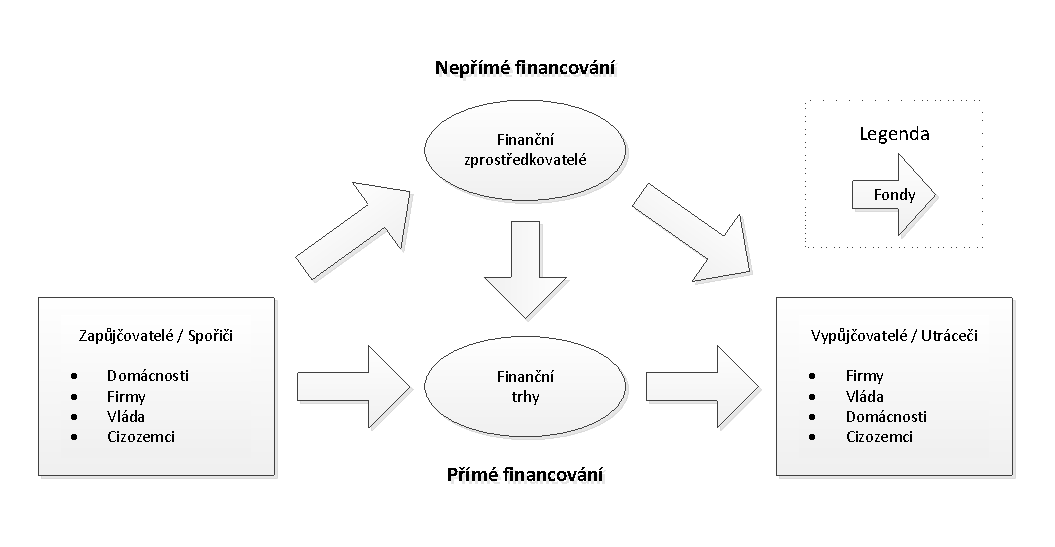
\includegraphics[width=\textwidth]{images/fintrh} 
	\caption[Přímé a nepřímé financování]{Přímé a nepřímé financování. Převzato z \cite{zakpriban}.}\label{fig:fintrh}
\end{figure}


% ----- %

\subsection{Typy finančních trhů}

Finanční trhy lze chápat různými způsoby, a proto je lze rozdělit podle různých hledisek. Níže jsou uvedená některá z nich.  
%\cite{zakfin}

\begin{enumerate}
	\item Podle typu obchodovaného instrumentu:
		\begin{itemize}
			\item dluhové trhy (např. obchodování s dluhopisy),
			\item akciové trhy (obchodování s akciemi).
		\end{itemize}
	\item Podle splatnosti instrumentu:
		\begin{itemize}
			\item peněžní trh (instrumenty se splatností do 1 roku, např. státní pokladniční poukázky),
			\item kapitálový trh (instrumenty se splatností nad 1 rok, např. akcie nebo dlouhodobé dluhopisy).
		\end{itemize}
	\item Podle obchodovatelnosti instrumentu:
		\begin{itemize}
			\item primární trh (instrumenty prodané prvotním investorům),
			\item sekundární trh (obchodování s již vydanými instrumenty).
		\end{itemize}
	\item Podle organizace trhů:
		\begin{itemize}
			\item burzovní trhy (vysoce standardizované obchody probíhající za jedinou cenu, např. NYSE nebo BCPP),
			\item mimoburzovní trhy (oproti burzovním trhům nižší standardizace obchodů a cena instrumentů 
				obvykle různá pro nákup a prodej, např. NASDAQ).
		\end{itemize}
\end{enumerate}

V následujících oddílech jsou popsány trhy, které mají spojitost s tématem této diplomové práce a projektu, 
jehož je tato práce součástí.

% ----- %

\subsection{Kapitálové trhy}

Podnik získává kontaktem s kapitálovým trhem možnost financovat svoji expanzi a přijímat i rizikovější projekty. Kapitálový 
trh charakterizuje individualizace rizika. Díky tomu je schopen financovat i podnikatelské záměry, na kterých se banky 
nechtějí podílet, a jejichž možný výnos současně odpovídá míře podstupovaného rizika. Kapitálový trh tedy vede k vyšší 
výkonnosti zúčastněných subjektů. %\cite{mekat}

Na kapitálovém trhu se obchodují dlouhodobé finanční instrumenty s dobou splatnosti obvykle přesahující 1 rok. Hlavními 
instrumenty obchodovanými na kapitálovém trhu jsou zejména akcie a dlouhodobé dluhopisy, proto bývá tento trh někdy 
nazýván trhem cenných papírů, ačkoliv cenné papíry mohou být i krátkodobé. %\cite{mekat} 

Cenný papír představuje pohledávku vlastníka 
vůči tomu, kdo jej vydal, a současně k němu vytváří právní nárok. Pro investory je velkou předností cenných papírů, 
že jsou velmi snadno převoditelné, a proto je možné je kdykoliv v případě potřeby prodat a získat za ně peněžní prostředky. 
%\cite{vseanal, mekat}

Obchody na kapitálových trzích jsou téměř vždy realizovány s pomocí finančních zprostředkovatelů. %\cite{mekat}

% ----- %

\subsection{Burzovní trhy}

Na burzovních trzích jsou obchody vysoce standardizovány a probíhají za jedinou cenu. Místem, kde k těmto obchodům 
dochází, jsou \textit{burzy}, které organizují trh s určitými instrumenty. Na burze se setkávají zájemci o nákup a prodej 
daného instrumentu. Jediná cena, za kterou jsou uskutečňovány obchody, zároveň utváří jeho cenu. %\cite{zakfin} 

Zatímco v minulosti bylo předmětem obchodu na burzách především různé zboží, později začaly vznikat specializované 
burzy a dnes jsou nejdůležitějšími obchodovanými instrumenty cenné papíry. \cite{hebu}

Burza musí zveřejňovat informace důležité pro investory, mezi které patří vlastní výroční zprávy, kurzy obchodovaných 
instrumentů či objemy obchodů. Burza dále musí zveřejňovat informace o členech burzy a samozřejmě burzovní pravidla. 
Důležitým indikátorem o vývoji kurzů cenných papírů jsou tzv. burzovní indexy. Ty zohledňují kurzy vybrané skupiny cenných 
papírů podle definovaných vztahů a souhrnně charakterizují tyto cenné papíry pomocí jediného ukazatele. Mezi 
nejvýznamnější světové indexy patří \textit{Dow Jones Industrial Average} či indexy \textit{Standard\&Poor's}, 
z domácích je to Index PX Burzy cenných papírů Praha. %\cite{mekat}

% Teď by se ještě daly popsat různý specifika burzovních obchodů (\cite{mekat}), ale to mi přijde už trochu zbytečný, 
% o tom bude pojednávat hned další podkapitola Obchodování na burze

% ----- %

\subsection{Akciové trhy}
	
Akcie, investiční instrument obchodovaný na akciovém trhu, je cenný papír, s nímž jsou spojena práva akcionáře na 
řízení společnosti, jejím zisku a na likvidačním zůstatku při jejím případném zániku. Akciová společnost získává 
prodejem svých akcií kapitál. K akcionáři, který se koupí akcií stává spolumajitelem akciové společnosti, naopak 
plynou finanční toky ze společnosti ve formě vyplácených dividend. Výše dividendy závisí na ekonomických výsledcích 
společnosti a na rozhodnutí valné hromady. \cite{htsmw} %zakfin

Vydání akcií se říká \textit{emise}. Primární emise akcií (IPO) představuje veřejnou nabídku akcií prvotním investorům, 
jež se odehrává při vstupu společnosti na burzu. Zvýšení počtu obchodovaných akcií na burze upsáním dalšího balíku 
akcií se říká sekundární emise akcií.

Hodnotu akcie udává jedině trh, vlastník nezískává žádné právo na její zaplacení. Okamžité ceně akcie na burze se 
říká \textit{kurz}; závisí na skutečných i očekávaných výsledcích hospodaření společnosti, vývoji odvětví i celkovému stavu 
ekonomiky. Kurz akcie je vytvářen na základě nabídky a poptávky mezi investory. \cite{prknab} %zakfin

Kromě burzovních trhů s cennými papíry je možné obchodovat s akciemi i na mimoburzovních trzích. Standardizace 
obchodů je u nich podstatně nižší než v případě burzovních trhů a obvykle se na nich obchodují cenné papíry, které 
nesplňují přísnější podmínky burzovního obchodování. Přesto se však některé organizované mimoburzovní trhy vyvinuly 
natolik, že představují plnohodnotné trhy cenných papírů. Příkladem takových trhů jsou například český RM-systém 
nebo americký NASDAQ. %\cite{zakfin, vseanal}

% --------------------------------- %

\section{Obchodování na akciové burze}
\label{sec:13}

Obchody na akciových burzách probíhají prostřednictvím licencovaných obchodníků zvaných členové burzy především 
z řad významných bank a makléřských firem. Tito obchodníci provádějí na přání svých klientů operace na akciových 
trzích, za což jim náleží odměna neboli provize.  \cite{prknab}

Na burze může působit tzv. \textit{tvůrce trhu}, kterým je člen burzy s platným oprávněním. Jeho účelem je zajišťovat 
dostatečnou \textit{likviditu} cenných papírů v nabídce a poptávce podáváním vlastních nákupních a prodejních objednávek. 
Tvůrce trhu tedy na rozdíl od licencovaných obchodníků zprostředkovávajících obchody za své klienty hraje aktivní 
roli a obchoduje na burze svým jménem a za své peníze.  \cite{htsmw} %vseanal

\subsection{Typy objednávek}

Burzy obvykle nabízejí několik typů nákupních a prodejních objednávek, další varianty mohou nabízet svým klientům 
členové burzy. Dále jsou uvedeny některé obvyklé typy objednávek. 

\subsubsection{Limitní objednávky}

Limitní objednávky jsou takové objednávky, které mají být provedeny za specifikovanou \textit{limitní cenu} nebo lepší.
%\cite{vseanal}

\subsubsection{Tržní objednávky}

Tržní objednávky jsou nákupní nebo prodejní příkazy bez uvedení ceny. Takové objednávky jsou párovány za nejlepší 
dostupnou cenu na trhu. %\cite{vseanal, psekont}

\subsubsection{Stop objednávky}

Stop objednávky jsou nadstavbou nad předchozími typy objednávek, rozeznáváme tedy stop limitní a 
stop tržní objednávky. Tyto příkazy obsahují cenu zvanou \textit{stop limit}. K aktivování objednávky dojde až poté, 
co kurz dané akcie dosáhne zadaného stop limitu (jeho překročení u stop nákupní objednávky či pokles pod něj 
v případě stop prodejní objednávky). % \cite{vseanal, psekont}

Nejdůležitějším příkladem stop objednávky je tzv. pokyn \textit{stop-loss} určený k prodeji akcií v případě, že jejich 
kurz poklesne pod stanovenou hranici. Obchodník se jeho podáním brání před rizikem, že by při náhlém poklesu kurzu 
jím vlastněných akcií utrpěl větší ztrátu, než je ochoten podstoupit.

\subsubsection{Objednávky \uv{Iceberg}}

Objednávky typu Iceberg umožňují automaticky rozložit objednávku velkého objemu do většího počtu postupně 
prováděných objednávek menšího objemu. Tyto příkazy obsahují množství zvané \textit{peak}, které udává maximální 
objem aktivní části objednávky. Jakmile je část objednávky s tímto množstvím zcela uspokojena, je automaticky vložena 
nová, opět s maximálním množstvím \textit{peak}. Takto je velká objednávka \textit{Iceberg} \uv{rozpouštěna}, dokud 
není celá zobchodována. 

Smyslem objednávek \textit{Iceberg} je, aby se trh nedozvěděl o jejich celkovém objemu. Z tohoto důvodu nejsou 
aktivní části objednávky \textit{Iceberg} nijak rozlišeny od běžných objednávek. %\cite{vseanal}

% ----- %

\subsection{Obchodní den burzy}

Obchodní den burzy se skládá z předobchodní fáze, hlavní obchodní fáze a poobchodní fáze.

V předobchodní fázi, jíž začíná burzovní den, probíhá sběr objednávek. Obchodníci mohou vkládat objednávky do 
knihy objednávek, měnit je i rušit. Množství obchodních informací poskytovaných burzou v této fázi bývá omezeno, 
často je zveřejněn pouze závěrečný kurz daného akciového titulu z~předchozího obchodního dne. 

Během hlavní obchodní fáze dochází k uzavírání obchodů způsobem popsaným v následujícím oddíle.

Obchodní den končí poobchodní fází, během níž probíhá zpracování uzavřených obchodů, zveřejňování výsledků a 
sběr objednávek na další obchodní den. %\cite{vseanal}

Na obrázku \ref{fig:obchodni-den} jsou znázorněny průběhy obchodního dne pro běžné modely obchodování.

\begin{figure}\centering
	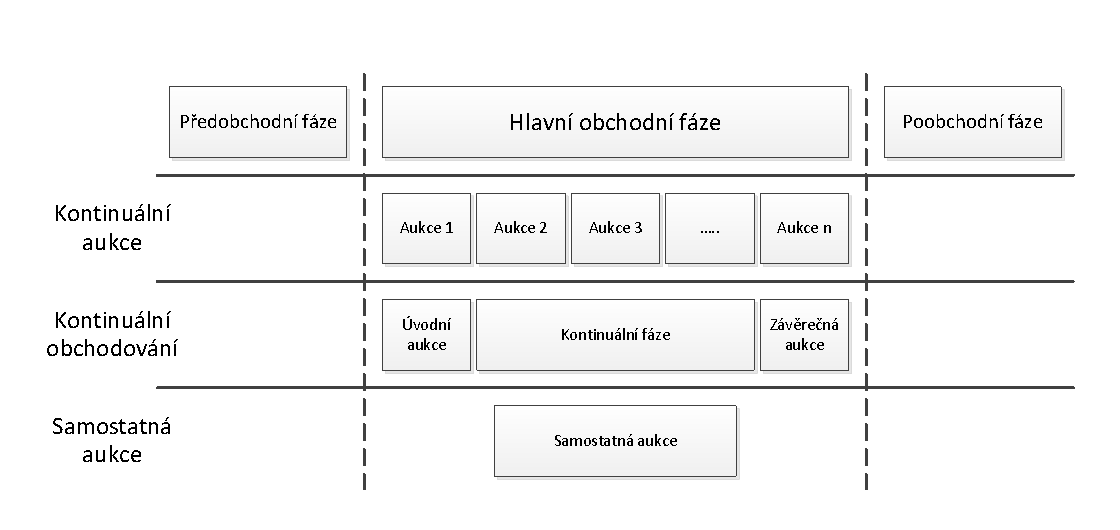
\includegraphics[width=\textwidth]{images/obchodni-den} 
	\caption[Modely obchodního dne]{Schéma obchodního dne burzy pro modely kontinuální aukce, 
			kontinuálního obchodování a samostatné aukce.}\label{fig:obchodni-den}
\end{figure}

% ----- %

\subsection{Způsoby utváření obchodů}

Existují dva základní způsoby obchodování na burze: aukce a kontinuální obchodování. Oba dva jsou níže podrobněji 
popsány. 


\subsubsection{Aukce}

Během obchodního dne může být realizována jedna nebo více aukcí, při nichž dochází k uzavírání obchodů. V průběhu 
aukce dochází na základě stanovených pravidel (která mohou být pro různé burzy odlišná) ke stanovení aukční ceny 
pro obchodovaný akciový titul. Následně jsou spárovány vhodné nákupní a prodejní objednávky zapsané v knize 
objednávek, na jejichž základě jsou za aukční cenu uzavřeny možné obchody. V případě, že není možné uspokojit 
všechny vhodné objednávky za danou aukční cenu, řídí se výběr spárovaných objednávek pravidly dané burzy.



\subsubsection{Kontinuální obchodování}

Hlavní obchodní fáze kontinuálního obchodování začíná úvodní aukcí a končí závěrečnou aukcí, během nichž jsou 
obchody uzavírány již popsaným způsobem. 

Mezi úvodní a závěrečnou aukcí probíhá kontinuální fáze, během níž dochází k průběžnému uzavírání obchodů na 
základě průběžně vkládaných objednávek podle stanovených pravidel. Každá nově vkládaná objednávka je 
ihned porovnána s objednávkami zapsanými v knize objednávek, a pokud to je možné, je ihned zobchodována.


% --------------------------------- %

\section{Přehled vybraných akciových burz}

V následujících oddílech jsou představeny některé světové burzy a platformy, na kterých jsou provozovány.

% ----- %

\subsection{Xetra}

Obchodní systém Xetra \cite{xetra} je obchodní platforma pro uskutečňování elektronických burzovních obchodů. 
Původně byl tento systém, provozovaný společností Deutsche Börse AG, vytvořen pro Frankfurtskou burzu, na které 
je nasazen od roku 1997, a později se rozšířil i na další burzy. Dnes platformu Xetra využívá např. vídeňská Wiener 
Börse AG nebo Burza cenných papírů Praha.

Přednostmi systému Xetra jsou především vysoká spolehlivost, rychlost prováděných transakcí a škálovatelnost. 
Platforma nabízí burzám jednotný a jednoduchý způsob obchodování, přičemž je vždy přizpůsoben pro specifické 
potřeby konkrétní burzy a legislativy platné v dané zemi.

Mezi základní vlastnosti systému patří:

\begin{itemize}
	\item Umožňuje obchodovat v režimech kontinuálního obchodování a samostatné a kontinuální aukce.
	\item Podporuje zadávání limitních, tržních a stop objednávek.
	\item V každém okamžiku existuje pro cenný papír pouze jedna cena.
	\item Obchodování je anonymní, obchodníci neznají své protistrany.
	\item Umožňuje působení tvůrce trhu.
	\item Při vypořádávání objednávek zohledňuje cenová a časová priorita.
	\item Kniha objednávek je během předobchodní fáze otevřená, v poobchodní fázi zavřená.
	\item Soubory s výsledky obchodování jsou vytvářeny každý den po ukončení poobchodní fáze.
\end{itemize}

Aukční cena je při aukci v systému Xetra stanovena podle následujících pravidel:

\begin{enumerate}
	\item Aukční cenou je cena, při níž dojde k uspokojení největšího objemu objednávek.
	\item Aukční cenou je cena, s nejmenším \textit{převisem} (rozdílem mezi nabízeným a poptávaným množstvím).
	\item Je-li převis ve všech případech na straně poptávky, je aukční cenou nejvyšší z potenciálně vyhovujících cen. 
		Je-li převis ve všech případech na straně nabídky, je aukční cenou nejnižší z potenciálně vyhovujících cen. 
	\item Aukční cenou je aritmetický průměr nejvyšší a nejnižší potenciálně vyhovující ceny.
	\item Je-li potřeba cenu vzniklou průměrováním zaokrouhlit, volí se nejbližší možná cena směrem k ceně 
		\textit{referenční} (ceně, za kterou byl cenný papír obchodován naposledy).
\end{enumerate}

% ----- %

\subsection{Euronext}

Burza Euronext \cite{euronext} vznikla v roce 2000 sloučením několika západoevropských burz s cílem využít jednotného 
trhu Evropské unie a stát se celoevropskou burzou, jež by zároveň byla jednou z největších burz na světě. Euronext 
dnes působí v Belgii, Francii, Nizozemsku, Portugalsku a Velké Británii. V roce 2007 se Euronext sloučil s americkou burzou 
NYSE a společně s dalšími menšími burzami tvoří skupinu NYSE Euronext. Od roku 2013 jsou tyto společnosti součástí 
Intercontinental Exchange \cite{ice}. 

Podobně jako u systému Xetra, i burza Euronext definuje základní pravidla \cite{euronextrules}, přičemž jednotlivé 
pobočky mají své vlastní upřesňující a doplňující soubory pravidel. Podporované jsou limitní, tržní i stop objednávky a 
jejich další modifikace. Provádění obchodů je možné v režimech kontinuálního obchodování a aukcí a taktéž mimo
obchodovací období. Při vypořádávání objednávek se zohledňuje striktní cenová priorita, avšak časová priorita už 
striktní není - někteří obchodníci v průběhu kontinuálního obchodování mohou mít při stejné limitní ceně vyšší prioritu 
než jiní.

Burza Euronext stanovuje aukční cenu při aukci podle následujících pravidel: 

\begin{enumerate}
	\item Aukční cenou je cena, při níž dojde k uspokojení největšího objemu objednávek.
	\item Je-li takových potenciálně vyhovujících cen více, je aukční cenou cena, jež je z nich nejblíže k ceně 
		referenční (ceně, za kterou byl cenný papír obchodován naposledy).
\end{enumerate}

% ----- %

\subsection{NYSE}

Newyorská burza NYSE \cite{nyse}, jejíž počátky sahají až do roku 1792, je dnes z~hlediska celkové tržní kapitalizace 
největší burzou obchodující s akciemi a deriváty na světě. Obchodování probíhá kombinovaným prezenčním způsobem 
s podporou elektronického systému. Kvůli tomu je kontrola uzavíraných obchodů značně problematická a zahrnuje několik 
úrovní dohlížitelů. Na burze působí kromě řadových obchodníků i tvůrci trhu, kteří udržují likviditu podáváním vlastních 
nákupních a prodejních objednávek. 

Burza NYSE podporuje kromě limitních, tržních a stop objednávek značné množství dalších odvozených typů. Zároveň 
zavádí množství různých \uv{statusů} pro obchodníky, kterým na jejich základě přísluší různé pravomoci a povinnosti. 
Objednávky jsou párovány s ohledem na cenovou a časovou prioritu a prioritu danou jejich typem. Žádná z těchto priorit
však není striktní a pravidla vypořádání obchodů jsou značně složitá.

V roce 2007 došlo ke spojení NYSE s evropskou burzou Euronext, od roku 2013 jsou tyto společnosti součástí sítě 
Intercontinental Exchange \cite{ice}. 


% --------------------------------- %


\section{Projekt simulátoru akciové burzy} 

Cílem projektu, jehož je tato diplomová práce součástí, je vývoj zjednodušeného simulátoru akciové burzy, na kterém bude 
možné provádět základní burzovní příkazy a sledovat vývoj kurzu obchodovaných akcií.

% ----- %

\subsection{Součásti projektu}
\label{sec:proj-parts}

Burza jako taková v našem případě sestává ze tří základních komponent: řídící aplikace Market, nástrojů pro výpočet aukční ceny
a párování objednávek Striker a databázového úložiště. Market je odpovědný za chod burzy, přijímá objednávky a další příkazy 
od členů burzy, informuje je o uskutečněných obchodech a odpovídá jim na dotazy. Nástroje Striker na žádost Marketu provádějí
výpočet aukční ceny požadovaného akciového titulu, párují nákupní a prodejní objednávky a informují Market o uzavřených 
obchodech. Market i Striker komunikují s databázovým úložištěm, ve kterém jsou uloženy všechny potřebné údaje pro chod burzy.

Klienti obchodují na burze prostřednictvím členů burzy, kterými jsou licencovaní obchodníci. Ti komunikují s Marketem, kterému 
podávají za své klienty objednávky, a poskytují svým klientům informace o jejich obchodech a celkové statistiky obchodů s akciemi.

Celkové schéma hlavních komponent burzy a jejích účastníků je zobrazeno na obrázku \ref{fig:global-schema}.

Předmětem této práce je schéma databázového úložiště burzy včetně řídících a obslužných procedur a nástroj Striker. Kolega 
Jan Jůna se ve své diplomové práci \cite{junadip} zabývá řídící aplikací burzy Marketem, obchodníky a klientským rozhraním.


\begin{figure}\centering
	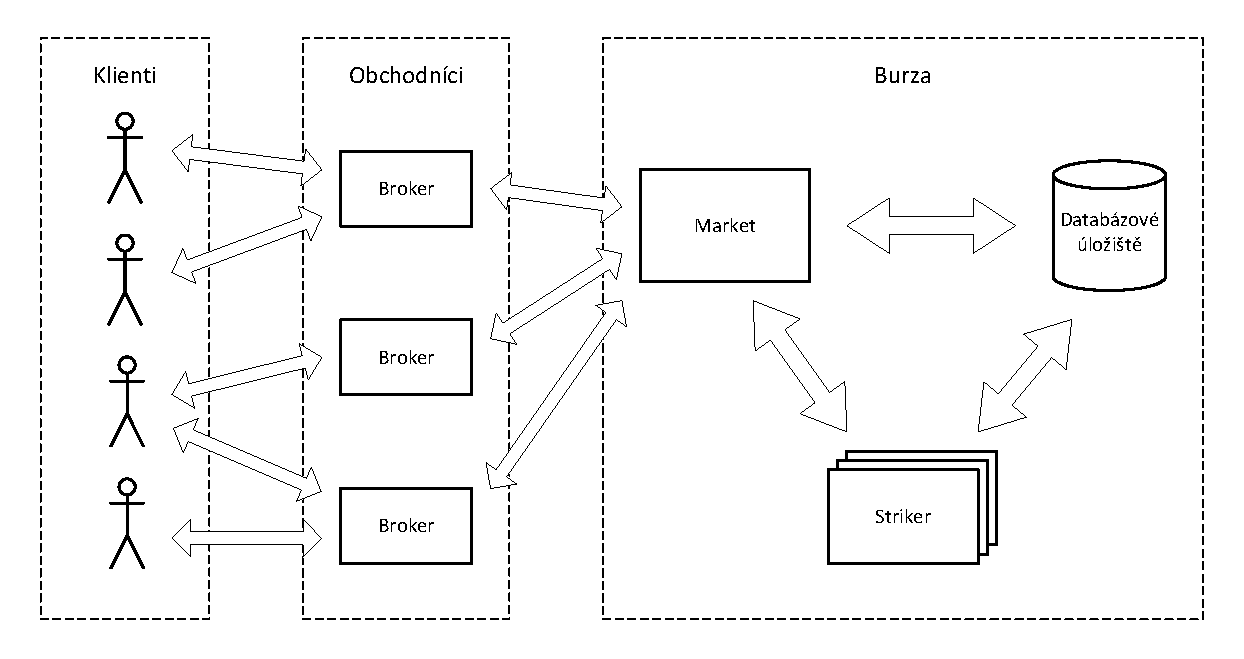
\includegraphics[width=\textwidth]{images/global-schema} 
	\caption[Schéma burzy]{Schéma hlavních komponent burzy a jejích účastníků}\label{fig:global-schema}
\end{figure}

% ----- %

\subsection{Terminologie používaná v projektu}

V následujících částech této práce budou používány pro vyvíjené komponenty projektu názvy představené již v předchozí podkapitole 
\ref{sec:proj-parts}. Níže následuje jejich formální specifikace.

\textit{Striker} bude nástroj pro výpočet aukční ceny a párování objednávek vyvíjený v rámci této této práce. 

\textit{Databáze} bude databázové úložiště vyvíjené v rámci této této práce. K~databázi budou mít přístup pouze Market a nástroje Striker.

\textit{Burza} bude představovat vyvíjenou burzu sestávající z Marketu, Strikerů a databáze. 

\textit{Market} bude řídící aplikace burzy. Bude komunikovat s databází, Strikery a obchodníky.

\textit{Obchodník} bude člen burzy oprávněný přímo obchodovat na burze. Jeho prostřednictvím budou obchodovat i jeho klienti. 
Obchodníci budou jedinými vnějšími subjekty, které bude burza znát.

\textit{Klient} v terminologii burzy nebude existovat, protože každý klient bude zastoupen svým obchodníkem. Z pohledu burzy 
všechny klientské příkazy bude vydávat obchodník, jemuž burza bude přisuzovat i vlastnictví všech jím spravovaných akcií. Vztah 
mezi obchodníkem a jeho klienty má na starosti sám obchodník (ve skutečnosti samozřejmě i kontrolní a regulační autority).


% ----- %

\subsection{Akceptovatelný rozsah funkčnosti} 

Projekt simulátoru akciové burzy počítá s mnoha zjednodušeními oproti skutečným burzám a zaměřuje se pouze na implementaci 
základních burzovních funkcí a procesů. 

Jedním ze zjednodušení je již samotný rozsah projektu, ve kterém vystupují tři aktéři: burza, obchodníci a jejich klienti. Ve skutečnosti 
je zúčastněných stran více. Na činnost burzy musí dohlížet kontroloři a vlastnictví akcií musí být evidováno patřičným úřadem 
(v případě České republiky jím je Centrální depozitář cenných papírů), kterému burzy musí předávat informace o~uskutečněných 
obchodech. Na skutečných burzách také obvykle figurují tzv. \textit{tvůrci trhu}, jejichž úkolem je zajišťovat dostatečnou 
likviditu podáváním nabídek a poptávek. 

Další důležitou roli hraje samotné vypořádání obchodů, kdy spolu s převodem akcií musí proběhnout i jejich zaplacení prodávající 
straně. Kromě toho musí být zaplaceny poplatky burze i obchodníkům a taktéž daně z prodeje akcií (v případě, že dojde k naplnění 
podmínek, jež stanovuje platná legislativní úprava). V reálném světě navíc dochází k vyplácení dividend a při určitých okolnostech 
může dojít k povinnému odkupu akcií. Všechny tyto aspekty v~našem projektu omezujeme pouze na samotný převod akcií.

Reálné burzy využívají několik typů objednávek, z nichž jsou nejběžnější limitní, tržní a stop objednávky. V rámci projektu 
simulátoru akciové burzy budeme podporovat pouze limitní objednávky. Další typy mohou být přidány v budoucích verzích.

Méně významným rozdílem bude obchodovaná jednotka. Reálné burzy obchodují v \textit{lotech}, přičemž jeden \textit{lot}
může představovat například 1000 kusů dané akcie, a objemy všech objednávek a tedy i obchodů jsou jeho celočíselným násobkem. 
Jelikož pro samotnou činnost burzy není obchodovaná jednotka podstatná, budeme pro jednoduchost ignorovat velikost lotu 
a obchodovat přímo s akciemi. Podobně budeme v případě databáze a Strikeru postupovat při operacích s údaji o ceně, kdy 
nebudeme vyjadřovat žádnou měnovou jednotku, díky čemuž budou tyto komponenty využitelné pro Market obchodující 
v libovolné měně. Stanovili jsme, že přesnost cenových údajů budeme udávat na 3 desetinná místa.

Ačkoliv se projekt týká přímo akciové burzy, burzovní obchodování s jinými cennými papíry se velmi podobá obchodování 
s akciemi. Nástroj Striker i databáze tak budou moci bez zásadních úprav pracovat i s ostatními instrumenty obchodovanými 
na kapitálové burze. Přesto s ohledem na terminologickou konzistenci s projektem simulátoru akciové burzy se bude v této
práci dále užívat pojmů obvyklých pro akciovou burzu.



% --------------------------------- %

\section{Specifikace požadavků}

V následujících oddílech jsou uvedeny klíčové požadavky kladené na vyvíjené řešení. Funkční požadavky zachycují nároky 
kladené na samotnou funkčnost aplikace, v nefunkčních požadavcích jsou shrnuty požadavky, které vymezují způsob 
jejího provedení a technologie, které mají být použity (v souladu s~rozdělením \cite{umlsroz}).

\subsection{Funkční požadavky}

\begin{enumerate}
	\item Databáze umožní zaznamenávat informace o obchodnících a obchodovaných akciových titulech.
	\item Databáze umožní zaznamenávat stav aktuálních nákupních a prodejních objednávek a již uzavřených obchodů.
	\item Databáze umožní uchovávat příkazy obdržené od uživatelů včetně časových údajů.
	\item Striker umožní Marketu zvolit akciový titul, pro který budou provedeny výpočty.
	\item Striker umožní načíst z databáze nevyřízené objednávky a další informace potřebné pro následující výpočty.
	\item Striker umožní spočítat aukční cenu zvoleného akciového titulu.
	\item Striker umožní uzavřít obchody spárováním nákupních a prodejních objednávek.
	\item Striker umožní uložit informace o uzavřených obchodech do databáze.
	\item Striker umožní vyrozumět Market o uzavřených obchodech.
\end{enumerate}

% ----- %

\subsection{Nefunkční požadavky}

\begin{enumerate}
	\item Databáze bude využívat databázového systému PostgreSQL verze 9 nebo vyšší.
	\item Všechny komponenty burzy budou komunikovat s databází výhradně přes uložené procedury (stored procedures). 
	\item Striker bude implementován v jazyce C++.
	\item Striker bude implementován tak, aby byl kód přenosný přinejmenším mezi následujícími POSIX platformami: OpenBSD, 
		FreeBSD, MacOSX, a Linux.
	\item Striker bude s ostatními komponentami burzy komunikovat pomocí protokolu TCP/IP.
	\item Striker bude navržen a implementován tak, aby jeho nároky na softwarové vybavení byly kromě požadovaných technologií minimální.
\end{enumerate}


% ------------------------------------------------------------------------------ %

\chapter{Analýza databázového úložiště}

\section{Základní přehled}

V této kapitole jsou shrnuty a rozpracovány základní požadavky na vlastnosti databáze. Rozsah práci je přitom omezen 
na potřeby Marketu a práci nástrojů Striker.


% --------------------------------- %

\section{Požadavky na databázi}

Z potřeb vyvíjené burzy vychází následující požadavky na entity uložené v databázi:

\begin{enumerate}
	\item Databáze uchová název společnosti, jejíž akcie jsou obchodovány na burze.
	\item Databáze umožní editovat údaje o evidovaných společnostech a přidávat nové.
	\item Databáze uchová pro obchodovaný akciový titul jeho plný a zkrácený název, společnost, jež tyto akcie vydala,
		datum první emise, celkový počet obchodovaných kusů a referenční cenu.
	\item Databáze umožní emisi akcií. Při emisi dojde k navýšení počtu obchodovaných kusů akcií tohoto titulu, 
		nastavení jeho referenční ceny na cenu stanovenou při emisi a k připsání emitovaných kusů emitentovi. 
	\item Databáze bude u registrovaných obchodníků evidovat jejich název a autentizační údaje.
	\item Databáze umožní editovat údaje o registrovaných obchodnících a přidávat nové.
	\item Databáze bude evidovat množství kusů jednotlivých akciových titulů ve vlastnictví (ve skutečnosti ve správě) obchodníků.
	\item Databáze umožní obchodníkům vkládat objednávky podporovaného typu. Obchodník u nich musí určit objednané množství 
		a akciový titul, jehož se objednávka týká, a v relevantních případech limitní cenu (pro limitní objednávky platí vždy). 
		U objednávky bude evidováno, kdy ji Market přijal a kdy byl obchodník informován o jejím přijetí. 
	\item Databáze umožní obchodníkovi zrušit podanou objednávku. 
	\item Databáze umožní Marketu zamítnout nebo expirovat podanou objednávku. 
	\item Databáze umožní obchodníkovi a Marketu sledovat stav objednávky. V~případě, že ji později obchodník zruší, 
		budou evidovány okamžiky přijetí příkazu ke zrušení a skutečného zrušení objednávky. Pokud dojde k~zamítnutí, 
		expiraci nebo vyřízení (uskutečnění obchodu s poslední zbývající částí) objednávky, bude zaznamenán i tento okamžik.
		Konečně, databáze bude evidovat i okamžik, kdy byl uživatel informován o ukončení objednávky (tedy
		vyřízení, expiraci, zrušení nebo zamítnutí).
	\item Databáze umožní zobrazit objednávky přijaté v zadaném časovém rozmezí.
	\item Databáze umožní zobrazit objednávky se zvoleným způsobem ukončení.
	\item Databáze umožní zobrazit objednávky, o jejichž stavu nebyl podávající obchodník informován.
	\item Databáze umožní zobrazit aktivní objednávky, tj. takové, které jsou relevantní při výpočtu aukční ceny a uskutečnění
		obchodů (viz \ref{sec:strikerorders}). 
	\item Databáze bude uchovávat uzavřené obchody. U těchto obchodů
		bude zaznamenávat, ze kterých objednávek pocházejí a kteří obchodníci tyto objednávky podali, aukční cenu, akciový 
		titul, jenž je předmětem obchodu, a jeho objem. Dále budou zaznamenány okamžiky, kdy došlo k~uzavření obchodu
		a kdy byli informováni prodávající a kupující obchodníci.
	\item Databáze umožní, aby byla objednávka rozdělena do více obchodů. Každý obchod však vzejde z právě jedné 
		nákupní a jedné prodejní objednávky.
	\item Databáze umožní synchronizované provedení všech obchodů uzavřených během aukce jednoho akciového titulu. 
		Při tom dojde k nastavení referenční ceny obchodovaného akciového titulu na aukční cenu, za níž byly obchody uskutečněny, 
		zaznamenání uzavřených obchodů a upravení zbývajícího množství v objednávkách účastnících se obchodu. Vlastnictví 
		zobchodovaných akcií bude převedeno z prodávajícího na kupujícího obchodníka.
	\item Databáze umožní zobrazit obchody vybraného obchodníka ve stanoveném časovém rozmezí.
	\item Databáze umožní Marketu uložit spočítané statistiky prodejů ve zvoleném období. Tyto statistiky budou pro každý akciový 
		titul obsahovat objem uzavřených obchodů, hodnotu objemu uzavřených obchodů (celkové množství převedených finančních 
		prostředků) a referenční cenu na konci tohoto období.
	\item Databáze umožní evidovat IP adresu a port dostupných nástrojů Striker.
\end{enumerate}

% --------------------------------- %

\section{Identifikace entit}

Analýzou požadavků kladených na databázi byla identifikována potřeba uchovávat entity, jež jsou společně se stručným popisem 
uvedeny v tabulce \ref{tab:entities}.

\begin{table}\centering
	\begin{tabular}{| l | p{9cm} |}\hline
		Název	 		& Popis								\tabularnewline \hline \hline
		Společnost		& Společnost mající své akcie upsané na burze.		\tabularnewline \hline
		Akciový titul		& Na burze obchodovaný akciový titul.				\tabularnewline \hline
		Obchodník		& Licencovaný obchodník obchodující na burze.		\tabularnewline \hline
		Typ objednávky	& Číselník možných typů objednávky. Podporované typy: nákupní nebo prodejní limitní objednávka.			\tabularnewline \hline
		Objednávka		& Podaná objednávka určitého typu na nákup či prodej jistého množství kusů některého akciového titulu.		\tabularnewline \hline
		Uzavřený obchod	& Kontrakt mezi prodávajícím a kupujícím obchodníkem na určité množství kusů akciového titulu za určitou cenu.	\tabularnewline \hline
		Vlastnictví		& Množství kusů určitého akciového titulu vlastněné určitým obchodníkem.						\tabularnewline \hline
		Statistika obchodů	& Statistika uskutečněných obchodů během určitého období.								\tabularnewline \hline
		Nástroj Striker	& Informace o dostupných nástrojích Striker.											\tabularnewline \hline
	\end{tabular}
	\caption[Seznam identifikovaných entit.]{Seznam identifikovaných entit.}
	\label{tab:entities}
\end{table}



V následujících oddílech budou popsány některé méně zřejmé vlastnosti vybraných entit.

% ----- %

\subsection{Objednávka}

Objednávka bude po svém vložení \textit{aktivní}, což znamená, že se ji burza bude snažit vyřídit uzavřením jednoho nebo více obchodů. 
V případě, že z této objednávky vzejde obchod, sníží se nabízené resp. poptávané množství akcií o~zobchodované množství. Zobchodováním 
celého nabízeného resp. poptávaného množství je objednávka vyřízena a přestává být aktivní.

Objednávce, která není aktivní, budeme říkat \textit{ukončená}. Objednávku je možné ukončit některým z těchto způsobů:

\begin{itemize}
	\item vyřízení, 
	\item zrušení, 
	\item expirování, 
	\item zamítnutí.
\end{itemize}

\textit{Vyřízení objednávky} jsme popsali výše. \textit{Zrušení objednávky} iniciuje obchodník, zatímco \textit{zamítnutí} Market. 
V případě, že objednávka nebude do předem stanovené doby ukončena žádným jiným způsobem, dojde k její \textit{expiraci}.

O ukončení objednávky je obchodník Marketem informován a odeslání tohoto oznámení je zaznamenáno.

% ----- %

\subsection{Uzavřený obchod}

Uzavřený obchod vznikne na základě jedné nákupní a jedné prodejní objednávky. V rámci obchodu dojde k převodu určitého množství kusů 
dané akcie z~vlastnictví prodávajícího obchodníka do vlastnictví kupujícího. Obchody budou vždy uzavřeny na maximální možné množství 
kusů, takže vždy alespoň jedna z objednávek účastnících se obchodu se stane jeho provedením vyřízenou.

Díky této skutečnosti bude možné jednoznačně identifikovat uzavřený obchod pomocí dvojice objednávek, jež se ho zúčastnily. 


% --------------------------------- %

\section{Vlastnosti atributů} 

Na základě vlastností reálných kapitálových burz (NYSE, Euronext, BCPP) 
jsme stanovili minimální požadavky na některé atributy identifikovaných entit.
Tyto požadavky jsou uvedeny v tabulce \ref{tab:attributes}.

\begin{table}\centering
	\begin{tabular}{| l | l | l |}\hline
		Entita	 		& Atribut		& Vlastnost (atribut musí být schopen uložit)		\tabularnewline \hline \hline
		Společnost 		& identifikátor	& Minimálně 1000 unikátních hodnot.			\tabularnewline \hline 
		Akciový titul 		& identifikátor	& Minimálně 1000 unikátních hodnot.			\tabularnewline \hline 
		Obchodník 		& identifikátor	& Minimálně 100 unikátních hodnot.			\tabularnewline \hline 
		Objednávka 		& identifikátor	& Minimálně miliardy unikátních hodnot.			\tabularnewline \hline 
		Obchod 		& identifikátor	& Minimálně miliardy unikátních hodnot.			\tabularnewline \hline 
		(všechny) 		& cena		& 10 platných cifer, přesnost 3 desetinná místa.	\tabularnewline \hline 
		Objednávka 		& přijata		& Přesnost 0,001 sekundy nebo menší.			\tabularnewline \hline 
	\end{tabular}
	\caption[Požadované vlastnosti vybraných atributů.]{Požadované vlastnosti vybraných atributů.}
	\label{tab:attributes}
\end{table}


% --------------------------------- %

\section{Logický model} 

Na obrázku \ref{fig:log-model} je zobrazen logický model vycházející z požadavků kladených na databázi. 
V modelu jsou zobrazeny identifikované entity se svými atributy (podtrženy jsou primární klíče) a naznačeny vztahy
mezi nimi pomocí notace Crow's Foot. \cite{umlsroz, dbsdim}  % nebo \cite{dbmod} 


\begin{figure}\centering
	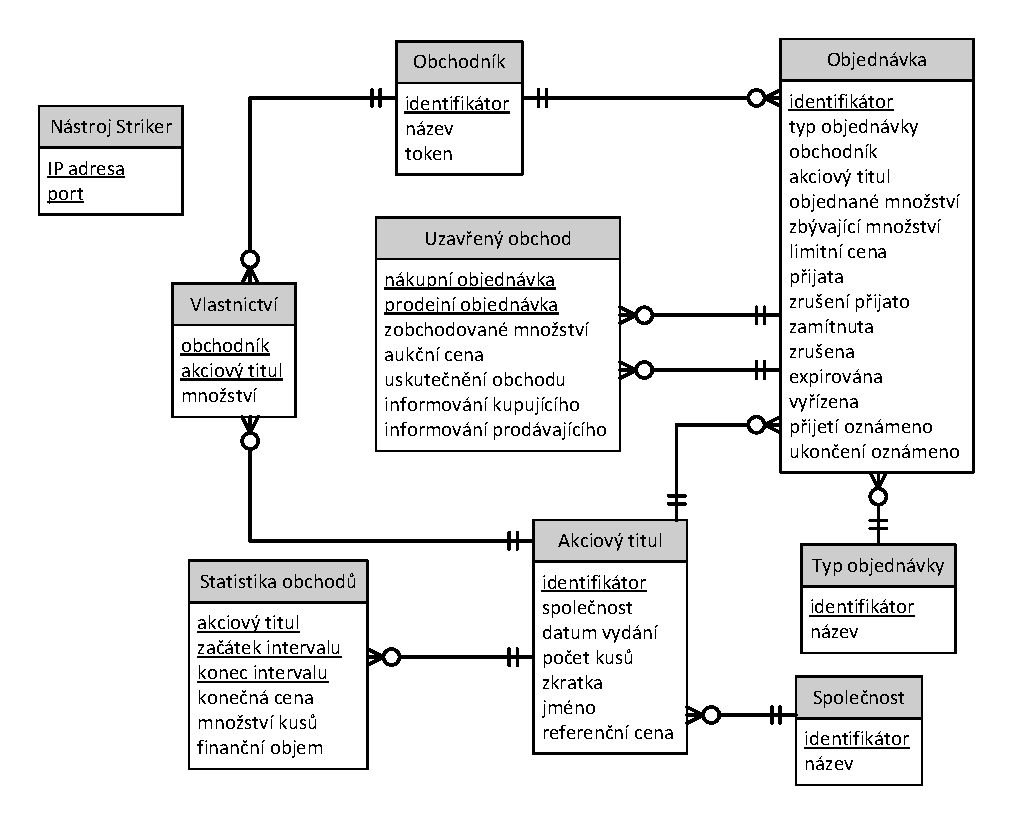
\includegraphics[width=\textwidth]{images/DB-log-model} 
	\caption[Logický model databáze]{Logický model databáze}\label{fig:log-model}
\end{figure}

% --------------------------------- %

\section{Uložené procedury}

Uložené procedury (\textit{stored procedures}) jsou databázové objekty, které umožňují obohatit databázi o vrstvu základní aplikační 
logiky a vlastní datové typy. Jedná se o metody vytvořené pomocí rozšířeného jazyka SQL nebo jiného programovacího jazyka podporovaného danou 
databází. S jejich pomocí je možné provádět všechny standardní databázové příkazy (např. \textit{SELECT} či \textit{INSERT INTO}) 
i složitější výpočty a operace.

Jedním z požadavků kladených na tuto práci je eliminace přímého přístupu ostatních součástí systému k datům uloženým v databázových 
tabulkách. Tento požadavek je podložen snahou o jednotný přístup k uloženým datům a zejména zapouzdření s nimi prováděných operací. 
Tím, že databáze nabídne ucelené rozhraní pro všechny procesy spojené s činností burzy, bude snazší zajistit zachování datové integrity 
a taktéž usnadní využití vyvíjeného databázového řešení i pro jiné burzy a jiné aplikace.

Potřebné uložené procedury je možné rozdělit do následujících kategorií podle jejich účelu:

\begin{itemize}
	\item provozní (vložit objednávku, zrušit objednávku),  
	\item vyhledávací (zobrazit všechny aktivní objednávky), 
	\item organizační (přidat společnost, upravit informace o obchodníkovi), 
	\item archivační (zadat, že obchodník byl informován o ukončení objednávky),
	\item prováděcí (provést obchody, provést emisi),
	\item pomocné (volané výhradně z jiných procedur).
\end{itemize}

Podrobnější popis vyžadují zejména prováděcí uložené procedury, jejichž oba zástupci jsou uvedeni v následujících oddílech.

% ----- %

\subsection{Provedení obchodů}
\label{sec:processtrades}

Vstupem procedury provádějící obchody bude seznam obchodů, které připravil Striker. Všechny tyto obchody se týkají jediného 
akciového titulu, proběhly tedy za stejnou aukční cenu a bude jim nastaven stejný okamžik zobchodování, totiž začátek běhu této 
funkce. 

Celá procedura probíhá v jediné transakci, neboť v žádném případě nesmí nastat situace, že by byly provedeny některé obchody 
a jiné nikoliv. Díky tomu zároveň nezáleží na pořadí provedených úkonů.

V průběhu provádění obchodů bude nastavena referenční cena akciového titulu na hodnotu aukční ceny obchodů (v případě, že 
není uzavřen žádný obchod a vstupní seznam obchodů je tedy prázdný, ke změně referenční ceny nedojde) a pro každý 
obchod proběhnou následující úkony:

\begin{itemize}
	\item zaznamenání obchodu,
	\item odečtení zobchodovaného množství akcií ze zbývajícího množství nákupní objednávky,
	\item odečtení zobchodovaného množství akcií ze zbývajícího množství prodejní objednávky,
	\item připsání zobchodovaného množství akcií do vlastnictví kupujícího obchodníka,
	\item odečtení zobchodovaného množství akcií z vlastnictví prodávajícího obchodníka.
\end{itemize}

Výstupem je pořízené časové razítko, a to i v případech, kdy není uzavřen žádný obchod. 

% ----- %

\subsection{Emise akcií}
\label{sec:emitstocks}

Emisi akcií bude možné provést dvojím způsobem: buď jako primární emisi akcií \cite{htsmw} nebo upsáním dalšího balíku akcií. 

V případě primární emise dojde nejprve k vytvoření záznamu o akciovém titulu vydaném emitující společností. Výstupem bude
vygenerovaný identifikátor akciového titulu. Druhým krokem bude postup identický s upsáním akciového titulu.

Úpis akciového titulu spočívá v navýšení již obchodovaného množství akcií o upisované kusy, nastavení referenční ceny na 
cenu úpisu a převodu těchto akcií emitentovi, který je v den emise nabídne k prodeji. 

% --------------------------------- %

\section{Komunikace s ostatními komponentami burzy}

V následujících oddílech jsou popsány nejdůležitější operace z hlediska komunikace jednotlivých komponent.

% ----- %

\subsection{Vložení objednávky}

Postup vložení objednávky je znázorněn na obrázku \ref{fig:seq-insert-order-anal}. Obchodník pošle svoji objednávku Marketu, který 
ji bez zbytečného prodlení předá databázi. V případě, že se podaří objednávku uložit, je jí přidělen jednoznačný identifikátor 
a ten je vrácen Marketu. Market pak informuje obchodníka o přijetí objednávky a vyplní atribut \textit{Přijetí oznámeno} 
objednávky zaznamenané v databázi aktuálním časovým razítkem.

\begin{figure}\centering
	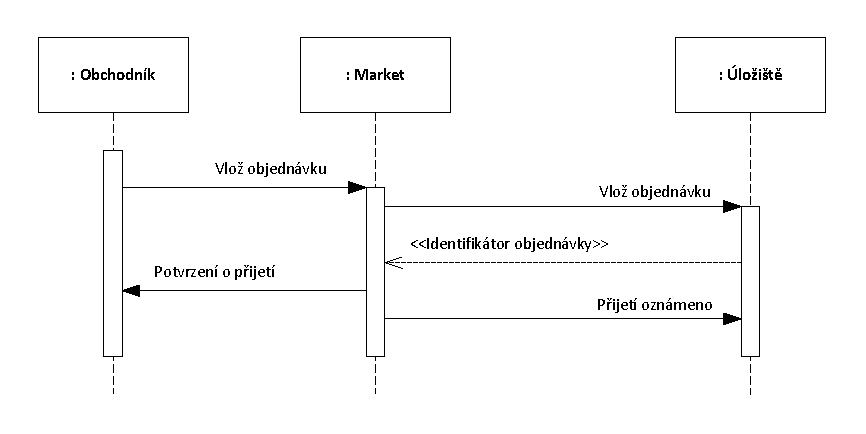
\includegraphics[width=\textwidth]{images/seq-insert-order-anal} 
	\caption[Diagram vložení objednávky]{Sekvenční diagram znázorňující vložení objednávky}\label{fig:seq-insert-order-anal}
\end{figure}

Market se může kdykoliv dotázat databáze na objednávky, které byly přijaty, ale jejich přijetí nebylo oznámeno. Obchodníkům, 
kteří tyto objednávky vložili, pak může odeslat chybějící oznámení a toto oznámení zaznamenat v~databázi.

Na rozdíl od rušení a expirace, které jsou popsány v dalších oddílech, je vložení objednávky možné i ve chvíli, kdy probíhá výpočet aukční 
ceny a párování objednávek, neboť na prováděné operace nemá vložená objednávka, jež se těchto operací neúčastní, žádný vliv.

% ----- %

\subsection{Zrušení objednávky}

Obchodník může požadovat zrušení vložené objednávky, jež dosud nebyla ukončena. Market ihned po obdržení takového příkazu zaznamená
požadavek zavoláním uložené procedury, která vyplní atribut \textit{Zrušení přijato} dané objednávky časovým razítkem a vrátí množství kusů, 
které z této objednávky dosud nebyly zobchodovány (a jichž se má zrušení týkat). Pokud zrovna Striker neprovádí výpočet aukční ceny 
a párování objednávek pro daný akciový titul, může být přistoupeno k samotnému zrušení (zbytku) objednávky. V~opačném
případě se musí počkat, až skončí výpočet, a teprve potom ji zrušit, pokud nebyla mezitím vyřízena.

Skutečné zrušení objednávky proběhne zavoláním patřičné uložené procedury, která objednávce vynuluje atribut \textit{Zbývající množství}, 
vloží časové razítko k atributu \textit{Zrušena} a jako výsledek vrátí počet kusů akcií, který u této objednávky zbýval do vyřízení. 
Market poté informuje obchodníka a vloží časové razítko k atributu \textit{Ukončení oznámeno}.

Komunikace mezi obchodníkem, Marketem a databází při rušení objednávky je znázorněna na obrázku \ref{fig:seq-cancel-order-anal}.

\begin{figure}\centering
	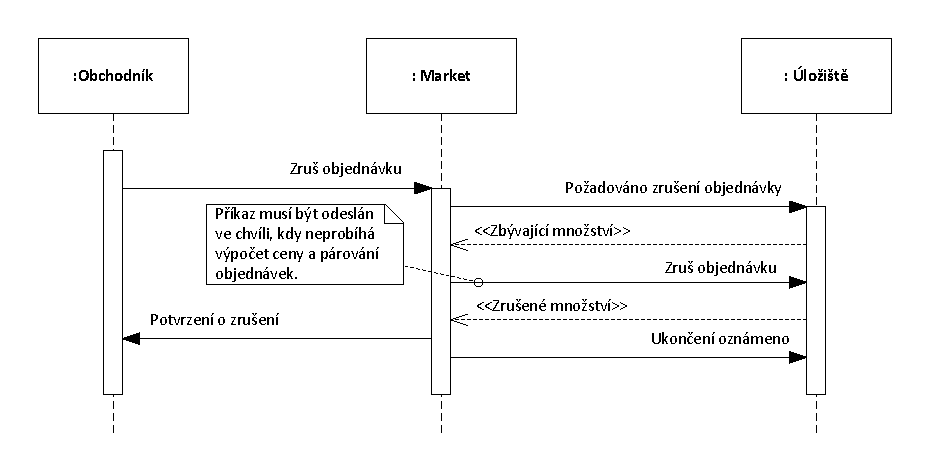
\includegraphics[width=\textwidth]{images/seq-cancel-order-anal} 
	\caption[Diagram zrušení objednávky]{Sekvenční diagram znázorňující zrušení objednávky}\label{fig:seq-cancel-order-anal}
\end{figure}

% ----- %

\subsection{Expirace objednávky}

Market by se měl v pravidelných intervalech dotazovat databáze na \uv{prošlé} objednávky, tedy takové, které byly vloženy před delší dobou,
než je životnost objednávky, stanovená při jejím zadání. 
Tyto objednávky postupně \textit{expirují}, což má stejné důsledky jako zrušení objednávky, pouze se nastavuje jiný atribut pro odlišení příčiny. 
Stejně jako pro rušení objednávky i zde platí, že objednávky mohou expirovat pouze v okamžiku, kdy pro daný akciový titul neprobíhá výpočet 
aukční ceny a párování objednávek.

Komunikace mezi obchodníkem, Marketem a databází při expiraci objednávky je znázorněna na obrázku \ref{fig:seq-expire-order-anal}.

\begin{figure}\centering
	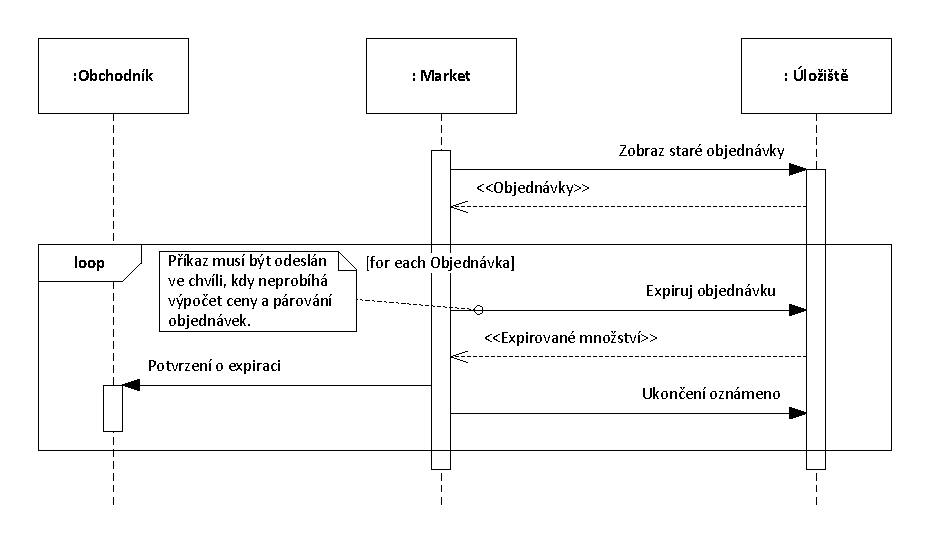
\includegraphics[width=\textwidth]{images/seq-expire-order-anal} 
	\caption[Diagram expirace objednávky]{Sekvenční diagram znázorňující expiraci objednávky}\label{fig:seq-expire-order-anal}
\end{figure}

% ----- %

\subsection{Výpočet a provedení obchodu}

Komunikace mezi Strikerem a databází je popsána v kapitole Analýza nástroje Striker \ref{sec:dbstrikercom}. 

% ------------------------------------------------------------------------------ %

\chapter{Analýza nástroje Striker}


\section{Základní přehled}

V této kapitole jsou shrnuty a rozpracovány základní požadavky na funkčnost nástroje Striker
a identifikovány základní procesy umožňující řešení požadované problematiky.


% --------------------------------- %

\section{Činnost nástroje}

Hlavním úkolem nástroje Striker je určování aukční ceny a párování objednávek pro akciový titul zadaný Marketem. Market může 
zadávat úkoly více Strikerům, jeden akciový titul však v daném okamžiku vždy počítá právě jeden Striker.

Jednotlivé činnosti Strikeru jsou zobrazeny na obrázku \ref{fig:striker-steps}. Tyto aktivity jsou dále podrobněji rozpracovány.


\begin{figure}\centering
	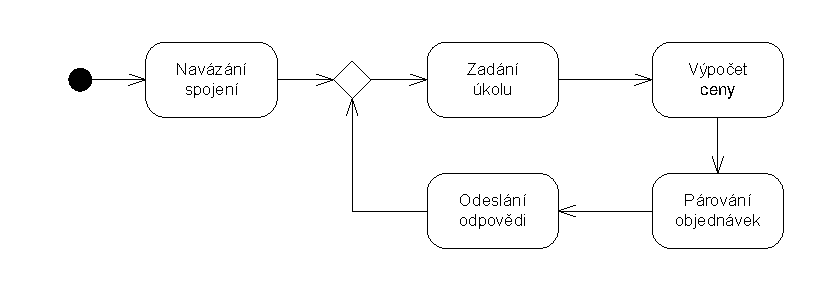
\includegraphics[]{images/striker-steps} 
	\caption[Sled činností Strikeru]{Sled činností Strikeru. Striker sám nikdy neukončuje svoji činnost.}\label{fig:striker-steps}
\end{figure}


% --------------------------------- %

\section{Komunikace s Marketem}

Komunikace mezi Strikerem a Marketem bude probíhat asynchronně pomocí protokolu TCP/IP. 

% ----- %

\subsection{Navázání spojení a autentizace}

Striker se po svém spuštění nejprve zaregistruje do databáze, z níž Market může vybírat mezi 
dostupnými Strikery. Striker pak ve vztahu k Marketu funguje jako služba, kterou může Market využívat. 
Market požádá Striker o~spojení, Striker provede autentizaci a v případě, že proběhne úspěšně, bude od něj dále přijímat úkoly. 
V případě neúspěšné autentizace bude spojení odmítnuto.

% ----- %

\subsection{Zadání úkolu}

Market zadá úkol Strikeru posláním zprávy obsahující identifikační údaj akciového titulu, pro nějž má být spočítána aukční 
cena a spárovány objednávky.

% ----- %

\subsection{Odeslání výsledku}
\label{sec:strikerresult}

Striker po ukončení výpočtu a uložení změn v databázi vyrozumí Market o~provedených operacích. Zpráva bude
obsahovat informace o aukční ceně a jednotlivých uzavřených obchodech tak, aby Market nemusel pro vyrozumění
obchodníků o této aukci získávat žádné další informace z databáze.

Zpráva bude ve vhodném formátu obsahovat tyto položky:

\begin{itemize}
	\item identifikátor akciového titulu,
	\item aukční cenu,
	\item objem uzavřených obchodů, 
	\item nejvyšší cenu nákupní objednávky po uzavření obchodů, 
	\item nejnižší cenu prodejní objednávky po uzavření obchodů, 
	\item časové razítko uzavření obchodů,
	\item dále pro jednotlivé obchody:
		\begin{itemize}
			\item identifikátor nákupní objednávky,
			\item identifikátor prodejní objednávky,
			\item identifikátor kupujícího obchodníka,
			\item identifikátor prodávajícího obchodníka,
			\item objem uzavřeného obchodu.
		\end{itemize}
\end{itemize}

Tato zpráva bude odeslána i v případě, že nedojde k uzavření žádných obchodů. 

Jestliže identifikátor akciového titulu nebude existovat nebo nebude platný, Striker místo standardní zprávy odešle Marketu 
chybovou zprávu.

% ----- %

\subsection{Ztráta spojení}

V případě, že selže spojení mezi Strikerem a Marketem, Striker bude znovu čekat na spojení (které opět proběhne včetně 
autentizace). Pokud se spojení přeruší v průběhu výpočtu, Striker nejprve dokončí výpočet aukční ceny a 
párování objednávek.


% --------------------------------- %

\section{Komunikace s databází}
\label{sec:dbstrikercom}

V pravidelných časových intervalech Market provádí aukci, během níž je z~došlých objednávek pro jednotlivé akciové tituly vypočítána aukční 
cena a jsou uzavřeny obchody. Tyto výpočty provádí nástroje Striker na žádost Marketu, předanou pomocí zprávy obsahující identifikátor 
akciového titulu. 

Striker z databáze přečte potřebné informace o akciovém titulu a relevantních objednávkách pro výpočet (více o jejich výběru 
pojednává oddíl \ref{sec:strikerorders}). Po provedení výpočtu Striker předá databázi seznam spočítaných obchodů, která je 
v jediné transakci provede způsobem popsaným v oddílu \ref{sec:processtrades} a vrátí časové razítko, jež uzavřené obchody obdržely jako čas 
uskutečnění obchodu. V~posledním kroku Striker pošle Marketu zprávu obsahující vypočítané obchody doplněné o časové razítko.

Postup při provedení obchodu z hlediska komunikace mezi zúčastněnými subjekty je znázorněn na obrázku \ref{fig:seq-process-trades-anal}.

\begin{figure}\centering
	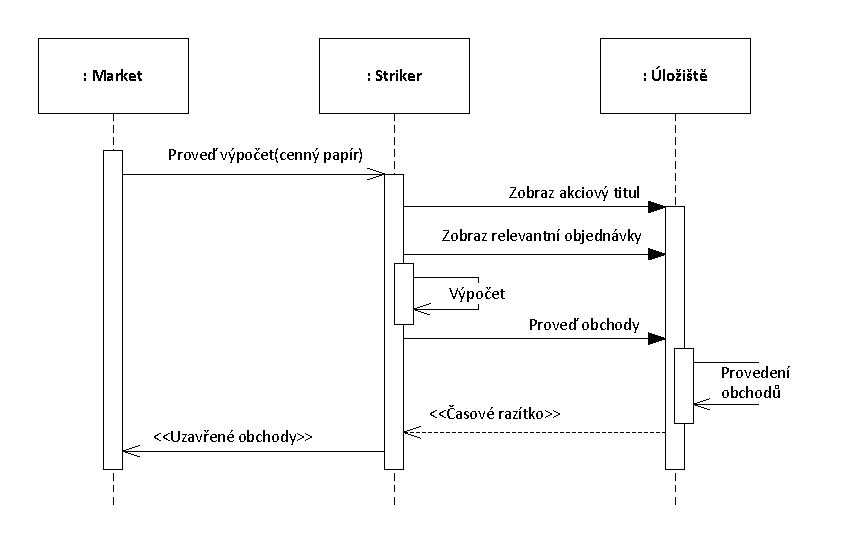
\includegraphics[width=\textwidth]{images/seq-process-trades-anal} 
	\caption[Diagram provedení obchodů]{Sekvenční diagram znázorňující provedení obchodů}\label{fig:seq-process-trades-anal}
\end{figure}

% --------------------------------- %

\section{Výpočet aukční ceny}

V následujících oddílech je podrobně rozebrán způsob stanovení aukční ceny akciového titulu na základě došlých objednávek.

% ----- %

\subsection{Kritéria}
\label{sec:strikercrit}

Pro stanovení aukční ceny akcie používáme algoritmus rozšířeného obchodního systému Xetra, jenž je popsaný např. v Pravidlech kontinuální 
aukce pražské burzy \cite{psekont}. 

\begin{enumerate}
	\item Maximalizace zobchodovaného objemu
	\item Minimalizace převisu 
	\item Směr převisu
	\item Průměrná cena
	\item Zaokrouhlení s přihlédnutím k referenční ceně
\end{enumerate}

% ----- %

\subsection{Výběr objednávek}
\label{sec:strikerorders}

Během aukce je dočasně pozastaven příjem objednávek, jakož i úpravy stávajících. Z knihy objednávek pro řešený akciový 
titul jsou vybrány všechny nákupní objednávky, jejichž limitní cena je vyšší nebo rovna nejnižší limitní ceně z prodejních
objednávek, a všechny prodejní objednávky, jejichž limitní cena je nižší nebo rovna nejvyšší limitní ceně z nákupních objednávek.

Těmto objednávkám říkejme \uv{relevantní}. Pouze tyto relevantní objednávky totiž mají vliv na stanovení aukční ceny akciového 
titulu a pouze tyto objednávky mohou být během probíhající aukce zobchodovány. Objednávky, které nejsou relevantní, zůstávají 
v knize objednávek a mohou být zobchodovány při následujících aukcích.

Jestliže kniha objednávek neobsahuje žádnou relevantní objednávku, nedojde k uzavření žádného obchodu a za aukční 
cenu je prohlášena cena referenční.

\subsubsection{Příklad výběru objednávek}

Předpokládejme, že burza přijala objednávky uvedené v tabulce \ref{tab:buysellorders}. Tyto objednávky jsou rozděleny 
na nákupní a prodejní, přičemž nákupní objednávky jsou řazeny podle limitní ceny sestupně a prodejní vzestupně. Jestliže
má více objednávek stejnou limitní cenu, je druhým kritériem při řazení v obou případech časový okamžik, kdy je burza přijala,
a podle něj jsou řazeny od nejstarších po nejmladší. 

V tabulce je pro lepší názornost místo časového razítka uvedeno pořadí, ve kterém byly přijaty. Objednávky, které podle výše 
popsaného způsobu nejsou relevantní (nemají vliv na stanovení aukční ceny akciového titulu), jsou označeny kurzívou.

\begin{table}\centering
	\begin{tabular}{|c|c|c||c|c|c|}\hline
		\multicolumn{3}{|c||}{Nákup}  & \multicolumn{3}{c|}{Prodej} \tabularnewline \hline 
		Pořadí	 	& Množství	& Cena	& Pořadí	& Množství	& Cena	\tabularnewline \hline \hline
		5		& 20		& 98		& 3		& 10		& 92		\tabularnewline \hline
		4		& 10		& 95		& 6		& 15		& 98		\tabularnewline \hline
		7		& 2		& 95		& \textit{1}	& \textit{25} & \textit{100} \tabularnewline \hline
		\textit{2}	& \textit{20} & \textit{90} & 		& 		& 		\tabularnewline \hline
	\end{tabular}
	\caption[Příklad obdržených objednávek]{Příklad obdržených objednávek. Kurzívou jsou označeny objednávky, které 
		nejsou relevantní, neboť jejich limitní cena je v případě nákupních objednávek příliš nízká a v případě
		prodejních objednávek příliš vysoká.}
	\label{tab:buysellorders}
\end{table}

% ----- %

\subsection{Sestavení tabulky}

Relevantní nákupní i prodejní objednávky vybrané způsobem popsaným v~předchozím bodě jsou využity k sestavení 
\textit{kumulativní tabulky}, s jejíž pomocí bude podle kritérií stanovena aukční cena.

První sloupec této tabulky tvoří jednotlivé limitní ceny obsažené v relevantních objednávkách. Pro každou cenovou hladinu je 
v dalších sloupcích uvedeno nabízené a poptávané souhrnné množství kusů akcií. Pro nákupní objednávky platí, 
že se jimi poptávané množství započítává všem cenovým hladinám nižším nebo rovné limitní ceně dané objednávky. Analogicky 
pro prodejní objednávky platí, že se jimi nabízené množství započítává všem cenovým hladinám vyšším nebo rovné limitní ceně 
takové objednávky.

Z relevantních objednávek uvedených v předchozím případě bude sestavena kumulativní tabulka \ref{tab:pricecalcex1}.

\begin{table}\centering
	\begin{tabular}{|c|c|c|c|c|}\hline
		Cena		& Nákup	& Prodej	& Obchod		& Převis	\tabularnewline \hline \hline
		\textbf{98} 	& 20 		& 25 		& \textbf{20} 	& 5 		\tabularnewline \hline
		95 		& 32 		& 10 		& 10 			& 22 		\tabularnewline \hline
		92 		& 32 		& 10 		& 10 			& 22 		\tabularnewline \hline
	\end{tabular}
	\caption[Příklad tabulky pro určení aukční ceny]{Příklad kumulativní tabulky pro určení aukční ceny. V této tabulce rozhodne
		o aukční ceně 1. kritérium. Aukční cena a rozhodující maximální zobchodovaný objem jsou zvýrazněny tučně.}
	\label{tab:pricecalcex1}
\end{table}

% ----- %

\subsection{Kritérium Maximalizace zobchodovaného objemu}

Prvním kritériem je maximalizace zobchodovaného objemu, tedy menší z poptávaného a nabízeného souhrnného množství akcií 
při zvolené aukční ceně. S~pomocí kumulativní tabulky jej pro každou cenovou hladinu spočítáme podle vzorce: 
\[obchod = \min(nákup, prodej).\] 

Jestliže je pro jedinou cenovou hladinu zobchodovatelný objem maximální, je tato cenová hladina prohlášena za 
aukční cenu. V opačném případě se použije druhé kritérium k výběru z těch cenových hladin, pro něž je zobchodovatelný
objem maximální.

Tabulka \ref{tab:pricecalcex1} ukazuje příklad, kdy je pro jedinou cenovou hladinu zobchodovatelný objem maximální (20), 
a proto se stává aukční cenou. Všechny uskutečněné obchody v této aukci tedy proběhnou za cenu 98 (zvýrazněna tučně).
O tom, které z relevantních objednávek budou zobchodovány, pojednává podkapitola \ref{sec:strikerpair}.

% ----- %

\subsection{Kritérium Minimalizace převisu}

V případě, že se nepodaří rozhodnout o aukční ceně na základě prvního kritéria, je na nejlepší kandidáty aplikováno kritérium
druhé, které upřednostňuje cenovou hladinu, při níž je převis minimální. Převisem se v tomto případě rozumí absolutní hodnota 
rozdílu mezi poptávaným a nabízeným množstvím akcií: 
\[převis = \left| nákup - prodej \right|.\] 

Jestliže je převis minimální pro jedinou cenovou hladinu z dříve vybraných, je tato cenová hladina prohlášena za aukční cenu. 
V opačném případě se přistupuje ke třetímu kritériu.

\begin{table}\centering
	\begin{tabular}{|c|c|c|c|c|}\hline
		Cena		& Nákup	& Prodej	& Obchod	& Převis		\tabularnewline \hline \hline
		98	 	& 20 		& 35 		& 20 		& 15	 		\tabularnewline \hline
		\textbf{95}	& 32 		& 20 		& 20 		& \textbf{12} 	\tabularnewline \hline
		\textit{92} 	& \textit{32}	& \textit{10}	& \textit{10}	&			\tabularnewline \hline
	\end{tabular}
	\caption[Příklad tabulky pro určení aukční ceny]{Příklad kumulativní tabulky pro určení aukční ceny. V této tabulce rozhodne
		o aukční ceně 2. kritérium. Řádek, který neprojde prvním kritériem, je označen kurzívou. Aukční cena a rozhodující 
		minimální převis jsou zvýrazněny tučně.}
	\label{tab:pricecalcex2}
\end{table}

Tabulka \ref{tab:pricecalcex2} je příkladem situace, kdy z prvního kritéria vzejdou dvě cenové hladiny: 98 a 95. Mezi nimi rozhodne
druhé kritérium, protože převis odpovídající ceně 95 je menší než v případě, kdy by aukční cenou byla cena 98. Cenová hladina 92
nepostoupila k vyhodnocení druhým kritériem, a proto pro ni převis není uveden.

% ----- %

\subsection{Směr převisu}

Pokud ani druhé kritérium nerozhodlo o aukční ceně, přistupuje se k porovnání \uv{směru} převisu finančního objemu cenových hladin,
jejichž převis byl podle minulého kritéria minimální. Pokud je převis na straně poptávky u všech zkoumaných cenových hladin (tedy
pokud ve všech případech převažuje poptávka nad nabídkou), je aukční cena rovna nejvyšší z těchto hladin. Pokud je naopak převis
na straně nabídky u všech zkoumaných cenových hladin (tedy ve všech případech převažuje nabídka nad poptávkou), je aukční cena
rovna nejnižší z těchto cenových hladin.

V případě, že pro některé cenové hladiny je převis na straně poptávky a pro jiné na straně nabídky, nelze podle tohoto kritéria 
rozhodnout a přistupuje se k dalšímu kritériu.

\begin{table}\centering
	\begin{tabular}{|c|c|c|c|c|}\hline
		Cena		& Nákup	& Prodej	& Obchod	& Převis		\tabularnewline \hline \hline
		\textit{98} 	& \textit{15}	& \textit{35}	& \textit{15}	& 	 		\tabularnewline \hline
		\textbf{95}	& 32 		& 20 		& 20 		& 12	 		\tabularnewline \hline
		92		& 32 		& 20 		& 20 		& 12		 	\tabularnewline \hline
	\end{tabular}
	\caption[Příklad tabulky pro určení aukční ceny]{Příklad kumulativní tabulky pro určení aukční ceny. V této tabulce rozhodne
		o aukční ceně 3. kritérium. Řádek, který neprojde prvním kritériem, je označen kurzívou. Mezi cenami 95 a 92 rozhodne
		převaha poptávky nad nabídkou (Nákup > Prodej), proto bude aukční cena 95 (zvýrazněna tučně).}
	\label{tab:pricecalcex3}
\end{table}

V tabulce \ref{tab:pricecalcex3} je ilustrován příklad, kdy ani druhé kritérium nerozhodne. z prvního kritéria vzejdou cenové hladiny 
95 a 92. Jejich převis je stejný, a tak dojde k porovnání poptávky a nabídky podle třetího kritéria. V obou případech poptávka převažuje
nabídku, a proto je za aukční cenu zvolena větší z nich: 95.

% ----- %

\subsection{Kritérium Průměrná cena}

Čtvrtým kritériem, které se může uplatnit v rozhodovacím procesu, je průměrná cena z nejvyšší a nejnižší cenové hladiny vzešlé 
z předchozího kritéria. Jestliže tato průměrná cena je validní (je násobkem nejmenší měnové jednotky), je prohlášena za aukční 
cenu; v opačném případě rozhodne poslední, páté kritérium.

\begin{table}\centering
	\begin{tabular}{|c|c|c|c|c|}\hline
		Cena		& Nákup	& Prodej	& Obchod	& Převis		\tabularnewline \hline \hline
		98	 	& 20 		& 35 		& 20 		& 15	 		\tabularnewline \hline
		95		& 35 		& 20 		& 20 		& 15		 	\tabularnewline \hline
		\textit{92} 	& \textit{35}	& \textit{10}	& \textit{10}	&			\tabularnewline \hline
	\end{tabular}
	\caption[Příklad tabulky pro určení aukční ceny]{Příklad kumulativní tabulky pro určení aukční ceny. V této tabulce o aukční ceně 
		nedokáže rozhodnout ani 3. kritérium, ze kterého postupují cenové hladiny 98 a 95. Jejich průměrná hodnota je 96,5.
		V případě, že taková cena je možná (např. pokud nejmenší jednotka je 0,1 nebo 0,5), stává se tato cena aukční cenou.
		V opačném případě je podle 5. kritéria zaokrouhlena podle referenční ceny.}
	\label{tab:pricecalcex45}
\end{table}

V tabulce \ref{tab:pricecalcex45} je ilustrován příklad, kdy ani třetí kritérium nerozhodne. Z~prvního kritéria vzejdou cenové hladiny 
95 a 98. Jejich převis je stejně velký, ale opačného směru, proto se podle čtvrtého kritéria spočítá jejich aritmetický průměr. 
V případě, že je cena 96,5 možná (například pokud je nejmenší jednotka 0,1), stane se aukční cenou. (Na tomto místě je vhodné 
poznamenat, že za libovolnou cenu ležící uvnitř intervalu cenových hladin vzešlých ze třetího kritéria je možné uzavřít stejný objem
obchodů.)

% ----- %

\subsection{Kritérium Zaokrouhlení s přihlédnutím k referenční ceně}

Jestliže cena vzniklá průměrováním podle předchozího kritéria není násobkem nejmenší měnové jednotky, rozhodne o aukční ceně
cena referenční (cena, za kterou se daný akciový titul obchodoval naposledy).

\begin{itemize}
	\item Je-li referenční cena vyšší než cena vzniklá průměrováním, je za aukční cenu prohlášena nejbližší vyšší validní cena.
	\item Jinak je za aukční cenu prohlášena nejbližší nižší validní cena.
\end{itemize}

Pokud by v příkladu uvedeném v tabulce \ref {tab:pricecalcex45} byla nejmenší jednotka 1 a referenční cena by byla vyšší než 96,5
(uvažujme např. 99), bude za aukční cenu zvolena cena 97. Pokud by ve stejné situaci byla referenční cena nižší (např. 95), 
aukční cena bude 96.

% --------------------------------- %

\section{Párování objednávek}
\label{sec:strikerpair}

V následujících oddílech je podrobně rozebrán způsob, jakým dochází k párování nabídek a poptávek a realizování obchodů.

% ----- %

\subsection{Zobchodované objednávky}

Zobchodovány mohou být pouze objednávky, jimž budeme říkat \textit{vyhovující}. Jsou to všechny nákupní objednávky, jejichž limitní cena 
je vyšší nebo rovna aukční ceně, a prodejní objednávky, jejichž limitní cena je nižší nebo rovna aukční ceně. Jsou možné tři případy:

\begin{itemize}
	\item Celkové objemy vyhovujících nákupních a prodejních objednávek jsou shodné. Zobchodovány budou všechny vyhovující objednávky.
	\item Celkový objem vyhovujících nákupních objednávek je menší než prodejních. Zobchodovány budou všechny vyhovující nákupní 
		objednávky, některé prodejní objednávky nebudou (zcela) zobchodovány.
	\item Celkový objem vyhovujících prodejních objednávek je menší než nákupních. Zobchodovány budou všechny vyhovující prodejní 
		objednávky, některé nákupní objednávky nebudou (zcela) zobchodovány.
\end{itemize}

V případě, že není možné zobchodovat všechny vyhovující objednávky, je potřeba stanovit kritéria, podle kterých dojde k výběru 
těch, které budou vyřízeny. Posuzovány jsou zvlášť nákupní a prodejní objednávky. Těmito kritérii jsou:

\begin{enumerate}
	\item Limitní cena:
		\begin{itemize}
			\item V případě nákupních objednávek mají nejvyšší prioritu ty s nejvyšší limitní cenou.
			\item V případě prodejních objednávek mají nejvyšší prioritu ty s nejnižší limitní cenou.
		\end{itemize}
	\item Okamžik přijetí objednávky: V případě shodné limitní ceny mají vyšší prioritu dříve přijaté objednávky.
	\item Náhodný výběr: Shodují-li se dvě nebo více objednávek v limitní ceně i okamžiku přijetí, o jejich vzájemném pořadí rozhodne 
			náhodný výběr.
\end{enumerate}

% ----- %

\subsection{Možný způsob párování}

Párování je možné provést tak, že nejprve budou zvlášť seřazeny vyhovující nákupní a zvlášť prodejní objednávky podle výše uvedených 
kritérií. Objem obchodu, který je vždy uzavřen na základě jedné nákupní a jedné prodejní objednávky, bude roven menšímu množství
kusů z obou nejlepších objednávek a obě objednávky účastnící se tohoto obchodu budou zmenšeny o toto množství. Objednávky, jejichž
zbývající množství kleslo na 0, nazveme vyřízené a budou odebrány z fronty objednávek. Párovací cyklus se opakuje do té doby, než
jsou vyřízeny všechny nákupní nebo prodejní objednávky.

Uvedeným způsobem dojde k uzavření následujícího počtu objednávek \textit{t}:
\[t \in \langle \max(b, s), b + s - 1 \rangle,\] 

kde \textit{b} je počet zobchodovaných nákupních objednávek a \textit{s} je počet zobchodovaných prodejních objednávek.

Tabulka \ref{tab:orderstotrades} znázorňuje obchody uzavřené tímto párováním z objednávek uvedených v tabulce \ref{tab:buysellorders}.

\begin{table}\centering
	\begin{tabular}{|c|c|c|}\hline
		Nákupní objednávka	& Prodejní objednávka	& Množství	\tabularnewline \hline \hline
		5				& 3				& 10		\tabularnewline \hline
		5				& 6				& 10		\tabularnewline \hline
	\end{tabular}
	\caption[Příklad uzavřených obchodů]{Příklad uzavřených obchodů na základě objednávek uvedených v~tabulce \ref{tab:buysellorders}. 
			Jako číslo objednávky bylo použito pořadí přijetí dané objednávky.}
	\label{tab:orderstotrades}
\end{table}


\subsection{Nevyřízené objednávky}

Vyhovující objednávky, které nebylo možné spárovat, zůstávají společně s~\uv{ire\-le\-vantními} objednávkami v knize objednávek a mohou se
v budoucnu po přijetí dalších objednávek účastnit určení nové aukční ceny a být zobchodovány. 

Po uzavření objednávek dle předchozího bodu by kniha objednávek obsahovala objednávky uvedené v tabulce \ref{tab:restorders}.

\begin{table}\centering
	\begin{tabular}{|c|c|c||c|c|c|}\hline
		\multicolumn{3}{|c||}{Nákup}  & \multicolumn{3}{c|}{Prodej} \tabularnewline \hline 
		Pořadí	 	& Množství	& Cena	& Pořadí	& Množství	& Cena	\tabularnewline \hline \hline
		4		& 10		& 95		& 6		& 5		& 98		\tabularnewline \hline
		7		& 2		& 95		& 1		& 25		& 100		\tabularnewline \hline
		2		& 20		& 90		& 		& 		& 		\tabularnewline \hline
	\end{tabular}
	\caption[Příklad zbývajících objednávek]{Příklad knihy objednávek po uzavření možných obchodů za cenu 98. Je patrné, že v tuto
			chvíli není možné uzavřít žádný další obchod.}
	\label{tab:restorders}
\end{table}

% --------------------------------- %

\section{Datová analýza}

V následujících oddílech jsou uvedeny a rozebrány požadavky na zaznamenání specifických datových struktur, s nimiž bude nástroj pracovat.

% ----- %

\subsection{Zaznamenání objednávek}

Pro potřeby vyhodnocení a zpracování objednávek bude potřeba načíst nákupní a prodejní objednávky do vhodného datového 
úložiště. Jeho vhodná podoba je naznačena na obrázku \ref{fig:statdiagram-order}.

Základním prvkem bude objednávka obsahující všechny potřebné informace pro výpočet aukční ceny a párování objednávek. Jak 
bylo objasněno v~průběhu analýzy, mezi tyto informace nepatří okamžik jejího přijetí, neboť Striker získá tyto objednávky již seřazené 
a jejich pořadí zachová.

Nákupní a prodejní objednávky budou dvě samostatné kolekce obsahující seřazené objednávky odpovídajícího typu.

\begin{figure}\centering
	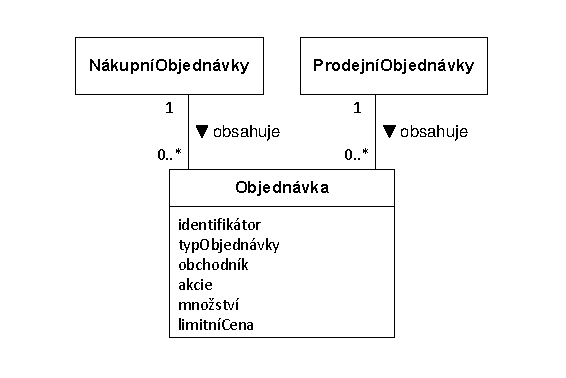
\includegraphics[]{images/statdiagram-order} 
	\caption[Statická struktura tříd pro zaznamenání objednávek]{Statická struktura tříd pro zaznamenání objednávek}\label{fig:statdiagram-order}
\end{figure}

% ----- %

\subsection{Uchování informací pro výpočet ceny}

Aukční cena bude určena pomocí kumulativní tabulky, jejímž základním prvkem je řádek charakterizovaný limitní cenou (v této práci se 
v kontextu kumulativní tabulky užívá pojmu \textit{cenová hladina}). Vhodná podoba této struktury je zobrazena na obrázku \ref{fig:statdiagram-pcr}.

Řádek tabulky obsahuje cenovou hladinu odpovídající limitní ceně některé objednávky a spočítané parametry potenciálního obchodu 
uzavřeného při této ceně.

\begin{figure}\centering
	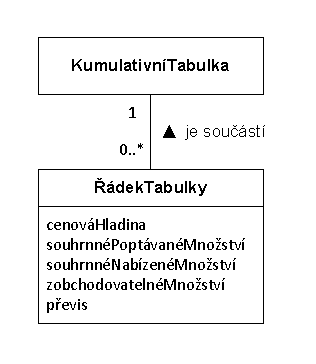
\includegraphics[]{images/statdiagram-pcr} 
	\caption[Statická struktura tříd pro uložení výpočet aukční ceny]{Statická struktura tříd pro uložení výpočet aukční ceny}\label{fig:statdiagram-pcr}
\end{figure}

% ----- %

\subsection{Zaznamenání obchodů}

Třída reprezentující uzavřené obchody musí obsahovat všechny potřebné informace pro provedení těchto obchodů. Na obrázku 
\ref{fig:statdiagram-trade} je znázorněno, že každý obchod sestává z jedné nákupní a jedné prodejní objednávky, přičemž každá
z těchto objednávek může být rozložena do více samostatných obchodů.

\begin{figure}\centering
	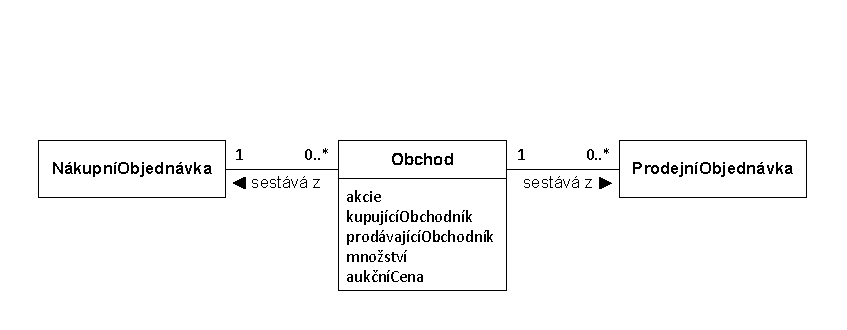
\includegraphics[]{images/statdiagram-trade} 
	\caption[Statická struktura tříd pro uložení obchodů]{Statická struktura tříd pro uložení obchodů}\label{fig:statdiagram-trade}
\end{figure}


% ------------------------------------------------------------------------------ %

\chapter{Návrh databázového úložiště}


\section{Základní přehled}

Tato kapitola logicky navazuje na analýzu databázového úložiště a zjištěné poznatky dále rozpracovává v jeho návrh.

Databáze bude postavena na objektově-relačním databázovém systému PostgreSQL \cite{postgres} verze 9.3.5; nebude-li to 
však na úkor efektivity, měl by být systém navržen tak, aby byl kompatibilní i se staršími verzemi. 


% --------------------------------- %

\section{Archivní a živé objednávky}

Analýza ukázala, že u přijatých objednávek bude potřeba evidovat značné množství informativních údajů z důvodů archivace historie, 
především různá časová razítka. Přitom bude potřeba provádět rychlé výpočty aukční ceny a následného párování objednávek, 
pro které bude potřeba napřed z databáze získat knihu objednávek. 

Vzhledem k očekávanému obrovskému množství uchovávaných objednávek, jejichž počet bude navíc neustále narůstat, by toto 
vyhledávání bylo značně neefektivní. Proto budeme objednávky evidovat ve dvou databázových tabulkách, a to jako 
objednávky archivní a živé.

Archivní objednávky budou obsahovat \uv{archivační} údaje, což jsou všechny atributy identifikované v analýze (viz obrázek 
\ref{fig:log-model}) kromě údaje \textit{zbývající množství} závislého na uskutečněných obchodech. 

Živé objednávky budou reprezentovat pouze aktivní objednávky, jež se mohou účastnit aukce, a pro tyto účely budou obsahovat 
pouze informace nutné k výpočtům a vytvoření obchodů. V okamžiku, kdy dojde k ukončení objednávky, bude tato objednávka 
smazána z tabulky živých objednávek.

Z výše uvedeného je zřejmé, že tabulka obchodů musí jako cizí klíč pro nákupní a prodejní objednávku používat tabulku archivních 
objednávek. Obchody se však vytvářejí z živých objednávek, a tak je nezbytně nutné, aby identifikátor jedné objednávky byl 
identický v tabulce archivních i živých objednávek.

Rozdělení objednávek na archivní a živé je dobře patrné porovnáním patřičné části logického \ref{fig:log-model} a 
fyzického \ref{fig:phy-model} modelu. 

% --------------------------------- %

\section{Tabulka obchodů}

V předchozí podkapitole již bylo konstatováno, že sloupce \textit{buy\_order\_id} a \textit{sell\_order\_id} představující nákupní resp. 
prodejní objednávku v tabulce obchodů musí odkazovat na tabulku archivních objednávek. 

Další změnou, kterou je oproti modelu vzešlého z analýzy vhodné provést, je přidání údajů o akciovém titulu a kupujícím a prodávajícím 
obchodníkovi. Tyto údaje jsou sice dostupné v odkazované tabulce archivních objednávek, ovšem z výše popsaných důvodů bude 
efektivnější vyhnout se pokud možno operacím s touto obří tabulkou. 

Pro snazší přístup k uzavřeným obchodům bude též každému obchodu přidělen jako jednoduchý primární klíč vlastní identifikátor, ačkoliv
by principiálně bylo možné použít kompozitní klíč složený z nákupní a prodejní objednávky, jak vzešlo z analýzy.

% --------------------------------- %

\section{Fyzický model}

V návrhu databázového úložiště byl vytvořen fyzický model databáze obsahující konkrétní tabulky včetně jejich sloupců 
s uvedenými datovými typy a informací, zda může obsahovat hodnotu \textit{NULL}, a dále primární a cizí klíče. Názvy tabulek i sloupců 
již odráží uvažované jmenné konvence. \cite{umlsroz} % nebo \cite{dbmod} 

Fyzický model navrhované databáze je zobrazen na obrázku \ref{fig:phy-model}. 

\begin{figure}\centering
	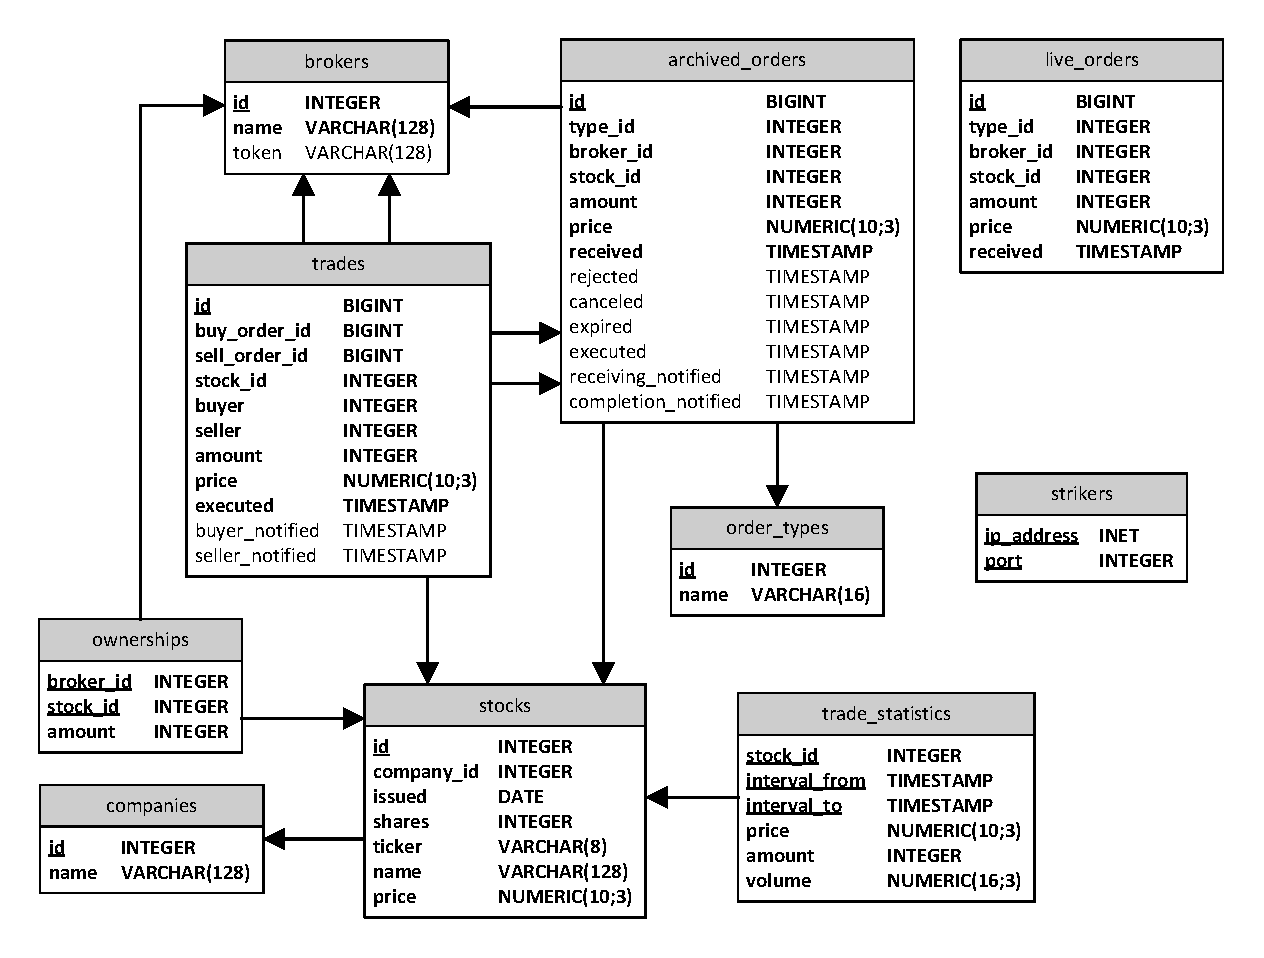
\includegraphics[width=\textwidth]{images/DB-phy-model} 
	\caption[Fyzický model databáze]{Fyzický model databáze. Podtržené názvy sloupců představují primární klíče tabulky, tučně jsou 
		označeny ty, jejichž hodnota nesmí být \textit{NULL}. Vazby cizích klíčů tabulky \textit{live\_orders} nejsou pro 
		lepší přehlednost vyznačeny.}\label{fig:phy-model}
\end{figure}

% --------------------------------- %

\section{Datové typy}

Datové typy jednotlivých sloupců databázových tabulek byly voleny s ohledem na požadovaný charakter ukládaných dat a jejich 
předpokládaný rozsah. 

% ----- %

\subsection{Celočíselné hodnoty}

Jelikož databázový systém PostgreSQL nepodporuje klasické bezznaménkové celočíselné datové typy \cite{pgdoc}, bude základním 
typem pro celočíselné hodnoty 32bitový datový typ \textit{integer}, jehož rozsah by měl být dostačující pro všechny uvažované sloupce 
s výjimkou identifikátorů objednávek a obchodů, pro něž bude použit 64bitový \textit{bigint}. 

Identifikátory společností, akciových titulů, obchodníků, objednávek a obchodů budou využívat automatického přidělování čísla, 
v termonologii systému PostgreSQL nazývaného \textit{serial types} \cite{pgdoc}. Tyto datové typy jsou ve skutečnosti normálními
celočíselnými typy, jimž je automaticky přidělováno pořadové číslo počínaje číslem 1, a proto jejich maximální hodnota je i přes jejich 
\uv{bezznaménkovost} stejná jako u mateřských datových typů. Pro identifikátor objednávek a obchodů bude použit typ \textit{bigserial}, 
v ostatních zmíněných případech \textit{serial}.

% ----- %

\subsection{Desetinná čísla}

Pro přesné vyjádření desetinných čísel lze v systému PostgreSQL využít datového typu \textit{numeric}, případně alternativního názvu 
\textit{decimal} \cite{pgdoc}. Pro zaznamenání ceny akcií bude ve všech případech využit \textit{numeric} s maximálním rozsahem 10 číslic, 
z toho 3 desetinných míst, a pro uchování údajů o hodnotě objemu obchodů v tabulce \textit{trade\_statistics} bude využit s rozsahem 
16 platných cifer při 3 desetinných místech.

% ----- %

\subsection{Řetězce}

Pro reprezentaci údajů ve formě čistého textu bude použit datový typ řetězce znaků proměnné délky \textit{varchar}. Maximální délka 
zkratky akciového titulu \textit{ticker} bude 8 znaků a název typu objednávky z číselníkové tabulky \textit{order\_types} bude omezen 
maximálně na 16 znaků. Délky ostatních řetězců vyskytujících se v databázi budou shodně omezeny na 128 znaků.

% ----- %

\subsection{Datum a čas}

S potřebou zaznamenávat časové údaje v databázi se setkáme u archivních i živých objednávek, u uzavřených objednávek a dále
u statistik obchodů. Ve všech těchto případech je potřeba evidovat datum a čas s co největší přesností. Systém PostgreSQL pro tyto 
účely poskytuje datový typ \textit{timestamp} ve variantách s nebo bez specifikování časového pásma \cite{pgdoc}. Pro jednoznačnou a přehlednou 
interpretaci uloženého údaje bude vyžadována ve všech případech varianta včetně časového pásma.

V tabulce \textit{stocks} bude dále nutné evidovat datum primární emise akcií (tzv. IPO). Pro tyto účely bude nejvhodnější datový typ
\textit{date}.

% ----- %

\subsection{Internetová adresa}

Databázový systém PostgreSQL definuje též několik speciálních datových typů pro reprezentaci síťových adres (viz \cite{pgdoc}). 
Pro zaznamenání IP adresy verze IPv4 nebo IPv6 v tabulce \textit{Strikers} bude použit datový typ \textit{inet}.

% --------------------------------- %

\section{Vložení objednávky}

Obchodníkovu objednávku vloží Market do databáze zavoláním uložené procedury \textit{insert\_order}. Tato funkce nejprve 
pořídí časové razítko, aby mohla nastavit shodný čas přijetí objednávky \textit{received} u živých i archivních objednávek, a ověří, 
že zadávané množství i limitní cena jsou kladná čísla. V případě prodejních objednávek je taktéž potřeba ověřit, že obchodník skutečně 
vlastní alespoň nabízené množství akcií daného titulu.

Poté již může být objednávka vložena do tabulky \textit{archived\_orders}, jež objednávce přiřadí identifikátor \textit{id}, nastaví 
okamžik vložení objednávky \textit{received} podle pořízeného časového razítka a hodnoty ostatních \uv{časových sloupců} ponechá 
\textit{NULL}. 

Databázový systém PostgreSQL využívá nadstavbu jazyka SQL, jež mimo jiné umožňuje vrátit hodnotu použitou v příkazu \textit{INSERT INTO} 
pomocí klíčového slova \textit{RETURNING} \cite{pgdoc}. S využitím této konstrukce bude možné efektivně použít identifikátor objednávky 
přidělený tabulkou \textit{archived\_orders} při následném vložení objednávky do tabulky živých objednávek \textit{live\_orders}.

Celá operace vložení objednávky bude probíhat v jediné transakci, čímž bude zaručeno správné zpracování objednávky. V případě, že 
objednávka bude přijata, vrátí metoda kladné číslo reprezentující identifikátor vložené objednávky. V opačném případě vrátí číslo 0 značící, 
že vložení objednávky selhalo.

%Procedurální jazyk PL/pgSQL \cite{pgplpgsql}

% --------------------------------- %

\section{Provedení obchodů}

Algoritmus provedení obchodů je podrobně popsán v analýze databázového úložiště \ref{sec:processtrades}. V této podkapitole bude dále 
rozpracován z hlediska návrhu provádějící metody \textit{process\_trades}.

Požadavek na provedení všech obchodů, nebo v případě selhání k neuskutečnění žádného, vede opět na nutnost provést celou operaci 
v rámci jediné transakce. 

Vstupem metody bude seznam spočítaných obchodů, jež je třeba provést. Pro tento účel bude potřeba vytvořit datovou strukturu 
\textit{t\_trade} reprezentující každý jednotlivý obchod, jež musí obsahovat prvky uvedené v tabulce \ref{tab:dbttrade}. Metoda 
\textit{process\_trades} pak bude přijímat parametr typu \textit{t\_trade[]}.


\begin{table}\centering
	\begin{tabular}{| l | l | l |}\hline
		Prvek					& Název		& Datový typ	\tabularnewline \hline \hline
		ID nákupní objednávky		& buy\_order\_id	& bigint		\tabularnewline \hline
		ID prodejní objednávky		& sell\_order\_id	& bigint		\tabularnewline \hline
		ID akciového titulu			& stock\_id		& integer		\tabularnewline \hline
		ID kupujícího obchodníka		& buyer\_id		& integer		\tabularnewline \hline
		ID prodávajícího obchodníka	& seller\_id		& integer		\tabularnewline \hline
		Obchodované množství		& amount		& integer		\tabularnewline \hline 
		Aukční cena				& price		& numeric(10, 3)	\tabularnewline \hline 
	\end{tabular}
	\caption[Struktura datového typu \textit{t\_trade}]{Struktura datového typu \textit{t\_trade}. ID značí identifikátor.}
	\label{tab:dbttrade}
\end{table}


Pro každý obchod typu \textit{t\_trade} bude vytvořen záznam v tabulce \textit{trades}, jenž bude dále obsahovat automaticky přidělený 
identifikátor a pro všechny obchody jednotné časové razítko pořízené metodou \textit{process\_trades} před začátkem zaznamenávání 
obchodů. Dále bude pro každý obchod aktualizován stav nákupní i prodejní objednávky voláním pomocné metody \textit{update\_order} a 
v případě, že kupující a prodávající obchodník budou rozdílní (jeden obchodník totiž může zastupovat prodávajícího i kupujícího klienta), bude
upraveno vlastnictví kupujícího a prodávajícího obchodníka pomocí metody \textit{increase\_ownership} resp. \textit{decrease\_ownership}.

Posledním krokem, který proběhne v případě, že byl uzavřen alespoň jeden obchod, bude aktualizování referenční ceny \textit{price} v tabulce
akciových titulů \textit{stocks}.

Metoda \textit{update\_order} sníží zbývající množství \textit{amount} aktivní objednávky uložené v tabulce \textit{live\_orders} o zobchodované 
množství. Pokud tímto obchodem byla objednávka vyřízena, bude daný záznam z tabulky \textit{live\_orders} smazán a odpovídajícímu záznamu 
v tabulce \textit{archived\_orders} (mají totožný identifikátor \textit{id}) bude nastaven parametr \textit{executed} na hodnotu okamžiku pořízení 
časového razítka uzavření obchodů.

Metody \textit{increase\_ownership} a \textit{decrease\_ownership} upraví vlastnictví akcií po uzavření obchodu. Jelikož tabulka \textit{ownerships} 
bude obsahovat z důvodu snížení množství ukládaných údajů pouze záznamy s nenulovým množstvím vlastněných akcií, mohou nastat tři různé 
situace.

\begin{enumerate}
	\item Záznam v tabulce \textit{ownerships} pro daného obchodníka a akciový titul před provedením obchodu neexistoval. V takovém případě 
		bude záznam vytvořen a množství vlastněných akcií \textit{amount} v tabulce \textit{ownerships} bude rovno nakoupenému množství
		\textit{\_traded\_amount}.
	\item V tabulce \textit{ownerships} před provedením obchodu již existuje záznam pro daného obchodníka a akciový titul a po jeho provedení
		množství vlastněných akcií \textit{amount} v tabulce \textit{ownerships} bude nenulové. Pak vztah vlastněného množství \textit{amount} 
		a zobchodovaného množství \textit{\_traded\_amount} bude následující: 
		\begin{itemize}
			\item \textit{amount} = \textit{amount} \(+\) \textit{\_traded\_amount} pro zvýšení vlastnictví a
			\item \textit{amount} = \textit{amount} \(-\) \textit{\_traded\_amount} pro snížení vlastnictví.
		\end{itemize}
	\item Po provedení obchodu bude množství vlastněných akcií \textit{amount} v tabulce \textit{ownerships} nulové. V takovém případě dojde
		ke smazání záznamu z tabulky \textit{ownerships}.
\end{enumerate}


% --------------------------------- %

\section{Emise akcií}

Vlastnosti emise akcií již byly rozebrány v průběhu analýzy \ref{sec:emitstocks}. Při jejím provádění bude potřeba rozlišit tzv. primární emisi (IPO), při které 
dojde k~vytvoření záznamu v tabulce akciových titulů \textit{stocks}, a úpisu dalšího balíku akcií, kdy dojde k navýšení počtu již obchodovaných akcií.

Úpis bude proveden pomocí uložené procedury \textit{emit}, jež v tabulce \textit{stocks} navýší počet obchodovaných kusů akcií \textit{shares} o počet 
upsaných kusů a nastaví referenční cenu \textit{price} na cenu úpisu. Dále dojde k navýšení vlastnictví \textit{ownerships} speciálního obchodníka 
\textit{Emitor} pomocí metody \textit{increase\_ownership} popsané v předchozí podkapitole (vzhledem k tomu, že databáze PostgreSQL nepodporují 
globální proměnné, bude pro přístup k obchodníkovi \textit{Emitor} využíváno volání metody \textit{emitor\_id()}, jež bude vracet jeho identifikátor). 

Primární emise akcií bude sestávat ze dvou kroků. V prvním kroku dojde k~vytvoření záznamu v tabulce \textit{stocks}, ve kterém budou vyplněny 
všechny údaje podle požadavku s výjimkou sloupce počtu obchodovaných kusů \textit{shares}, který bude nastaven na 0. Ve druhém kroku pak dojde 
k jeho navýšení na požadovaný počet a připsání akcií emitujícímu obchodníkovi voláním metody \textit{emit} jako při úpisu akcií. Primární emisi akcií bude 
provádět uložená procedura \textit{create\_stock}.

% --------------------------------- %

\section{Indexy}

% ----- %

\subsection{Základní vlastnosti indexů v systému PostgreSQL}

Indexy v databázových systémech slouží k urychlení vyhledání záznamů pomocí indexovaných sloupců při použití příkazů \textit{SELECT}, \textit{UPDATE} a 
\textit{DELETE}. Nevýhodou, kterou používání indexů obnáší, je větší režie při vytváření záznamů, kvůli níž nevhodně zvolený index nad málo používaným 
sloupcem může vést až k celkovému zpomalení práce s danou databází.

Indexy v databázovém systému PostgreSQL mohou být vytvořeny pro jednotlivé sloupce nebo (v případě některých typů indexů) pro více sloupců zároveň. 
Vícesloupcový index může být využit i pro vyhledávání s použitím jen některých sloupců daného indexu, ovšem jsou efektivní jen tehdy, pokud se daný výběr 
týká \uv{levých} sloupců uvedených v definici indexu. Je možná i opačná situace, tedy využití více jednosloupcových indexů při dotazu zahrnujícím několik sloupců.

Index je databází automaticky vytvořen pro všechny sloupce tvořící primární klíč a též omezení \textit{UNIQUE}. Obecně platí, že nebývá příliš výhodné 
používat indexy nad sloupci, které obsahují jen malou množinu různých hodnot.

O tom, zda bude index pro vyhledávání při konkrétním dotazu využit, nakonec rozhoduje vždy plánovač. Využití indexů v databázovém systému PostgreSQL 
je podrobně popsáno v dokumentaci. \cite{pgdoc}

% ----- %

\subsection{Identifikace častých dotazů}

Z vlastností indexů vyplývá, že pro správný výběr indexovaných sloupců je potřeba zjistit, které dotazy budou často prováděny. V tuto chvíli je možné na 
základě analýzy vytipovat možné kandidáty, ovšem správnost výběru se ověří až na základě statistik získaných při pilotním provozu s reálnými daty.

Kromě vyhledávání pomocí sloupců primárních klíčů a omezení \textit{UNIQUE}, pro které jsou indexy vytvořeny automaticky, lze očekávat, že kandidáty 
na vhodný index už budou pouze některé sloupce živých a archivních objednávek. 

\subsubsection{Živé objednávky}

Tabulka \textit{live\_orders} bude nejčastěji využívána k výpočtu aukční ceny a párování objednávek. Pro tyto výpočty bude potřeba vybírat zvlášť nákupní 
a prodejní objednávky jednoho akciového titulu a určité limitní ceny, přičemž pro určení maximální resp. minimální požadované ceny bude zapotřebí 
dotazu za účasti typu objednávky a akciového titulu. 

Jelikož navrhovaný systém alespoň zpočátku bude využívat pouze dva typy podobně četných 
objednávek, nedá se očekávat, že by indexace sloupce \textit{type\_id} byla přínosná. Naopak index složený ze sloupců \textit{stock\_id} a 
\textit{price} (v tomto pořadí) najde uplatnění při výběru objednávek pro výpočet i při výpočtu ceny pro uskutečnění tohoto výběru.

Dalším častým dotazem může být vyhledání všech živých objednávek zadaného obchodníka. Pokud budou tyto dotazy dostatečně využívány, bude vhodné 
indexovat i sloupec \textit{broker\_id}.

\subsubsection{Archivní objednávky}

Tabulka \textit{archived\_orders} bude sloužit především k archivaci údajů o přijatých objednávkách a nejčastěji k jejím údajům bude přistupováno pomocí 
identifikátoru indexovaného pomocí primárního klíče. Přesto se však dá očekávat nezanedbatelné množství dotazů týkajících se vyhledání určité podmnožiny
objednávek podané jedním obchodníkem nebo týkajících se jednoho akciového titulu.

Proto je navrženo využití jednoduchých indexů nad sloupci \textit{broker\_id} a \textit{stock\_id}.

\subsubsection{Uzavřené obchody}

Market umožní obchodníkům sledovat vývoj kurzu akcií v zadaném časovém intervalu. Pro tyto účely může být využita tabulka \textit{trade\_statistics} 
umožňující v době malého provozu (například po skončení obchodního dne) spočítat agregované statistiky obchodů ve zvolených časových intervalech. 

Tyto statistiky však budou plnit svůj účel pouze tehdy, pokud bude zvolený interval dostatečně široký. Pokud bude Market chtít znát tyto údaje v podrobnějším 
měřítku, bude je muset spočítat z uzavřených obchodů v tabulce \textit{trades}. Spočítané statistiky pravděpodobně nebude možné použít ani pro sledování 
kurzu v průběu aktuálního obchodního dne (tedy pokud se budou počítat až po jeho skončení), což jsou pro investory nejdůležitější informace.

Z uvedených důvodů se dá očekávat značné množství dotazů na tabulku \textit{trades}, ve které se bude vyhledávat pomocí sloupců \textit{stock\_id} a 
\textit{executed}. Proto bude vhodné použít složený index i na tuto dvojici sloupců. 

% ----- %

\subsection{Navržené indexy}

V tabulce \ref{tab:dbindexes} jsou uvedeny indexy, které budou využity v databázi. Tabulka obsahuje i automaticky vytvářené indexy při využití 
primárních klíčů a omezení \textit{UNIQUE}.

\begin{table}\centering
	\begin{tabular}{| l | l | l |}\hline
		Tabulka		& Sloupec	& Poznámka		\tabularnewline \hline \hline
		companies		& id		& Primární klíč	\tabularnewline \hline
		companies		& name	& Unique		\tabularnewline \hline
		stocks			& id		& Primární klíč	\tabularnewline \hline
		stocks			& ticker	& Unique		\tabularnewline \hline
		stocks			& name	& Unique		\tabularnewline \hline
		brokers		& id		& Primární klíč	\tabularnewline \hline
		brokers		& name	& Unique		\tabularnewline \hline
		order\_types		& id		& Primární klíč	\tabularnewline \hline
		archived\_orders	& id		& Primární klíč	\tabularnewline \hline
		archived\_orders	& broker\_id	& Index		\tabularnewline \hline
		archived\_orders	& stock\_id	& Index		\tabularnewline \hline
		live\_orders		& id		& Primární klíč	\tabularnewline \hline
		\multirow{2}{*}{live\_orders}	& stock\_id	& \multirow{2}{*}{Index}	\tabularnewline 
		 					& price	& 				\tabularnewline \hline
		live\_orders		& broker\_id	& Index		\tabularnewline \hline
		trades			& id		& Primární klíč	\tabularnewline \hline
		\multirow{2}{*}{trades}	& buy\_order\_id	& \multirow{2}{*}{Unique}	\tabularnewline 
		 				& sell\_order\_id	& 					\tabularnewline \hline
		\multirow{2}{*}{trades}	& stock\_id		& \multirow{2}{*}{Index}		\tabularnewline 
		 				& executed		& 					\tabularnewline \hline
		\multirow{2}{*}{ownerships}	& broker\_id	& \multirow{2}{*}{Primární klíč}	\tabularnewline 
		 					& stock\_id	& 					\tabularnewline \hline
		\multirow{3}{*}{trade\_statistics}	& stock\_id		& \multirow{3}{*}{Primární klíč}	\tabularnewline 
		 						& interval\_from	& 					\tabularnewline
		 						& interval\_to	& 					\tabularnewline \hline
		\multirow{2}{*}{strikers}	& ip\_address	& \multirow{2}{*}{Primární klíč}	\tabularnewline 
		 				& port			& 					\tabularnewline \hline
	\end{tabular}
	\caption[Navržené indexy]{Návrh na využití indexů v databázi. V~poznámce je uveden způsob vytvoření indexu. Každý řádek tabulky 
						představuje jeden index. V~případě, že je v jednom řádku uvedeno více databázových sloupců, jedná se 
						o~vícesloupcový index.}
	\label{tab:dbindexes}
\end{table}

% ------------------------------------------------------------------------------ %

\chapter{Návrh nástroje Striker}


\section{Základní přehled}

Tato kapitola logicky navazuje na analýzu nástroje Striker a zjištěné poznatky dále rozpracovává v jeho návrh.
Nástroj bude implementován v jazyce C++ jako program \texttt{striker}.


% --------------------------------- %

\section{Základní komponenty}

Vstupním bodem programu \texttt{striker} bude metoda \textit{main} nacházející se v souboru \texttt{Striker.cpp}. 
Tato metoda přečte dva parametry příkazového řádku, a to IP adresu a port, na kterých bude \texttt{striker} dostupný, 
a předá je konstruktoru třídy \textit{Striker}, jejíž vytvořená instance bude dál zodpovědná za řízení programu.

Nejdůležitější třídy podílející se na chodu programu jsou uvedeny v tabulce \ref{tab:apclsmain}, třídy reprezentující využité datové 
struktury jsou uvedeny v tabulce \ref{tab:apclssup}.

\begin{table}\centering
	\begin{tabular}{| l | l |}\hline
		Třída			& Úkol								\tabularnewline \hline \hline
		Striker	 		& Hlavní třída řídící chod programu.			\tabularnewline \hline
		TcpServer		& TCP server pro komunikaci s Marketem.		\tabularnewline \hline
		PgsqlDataProvider	& Výměna dat s databází.					\tabularnewline \hline
		JsonDataProvider	& Konverze dat do formátu JSON.			\tabularnewline \hline
		PriceCalculator	& Výpočet aukční ceny.					\tabularnewline \hline
		OrderMatcher	& Vytvoření obchodů spárováním objednávek.		\tabularnewline \hline
	\end{tabular}
	\caption[Hlavní třídy programu]{Nejdůležitější třídy podílející se na chodu nástroje Striker.}
	\label{tab:apclsmain}
\end{table}

\begin{table}\centering
	\begin{tabular}{| l | l |}\hline
		Třída				& Reprezentace			\tabularnewline \hline \hline
		Decimal 			& Desetinné číslo			\tabularnewline \hline
		Stock	 			& Akciový titul			\tabularnewline \hline
		Order	 			& Aktivní objednávka		\tabularnewline \hline
		Trade	 			& Obchod				\tabularnewline \hline
		PriceCalculationRow	& Řádek kumulativní tabulky	\tabularnewline \hline
	\end{tabular}
	\caption[Hlavní datové třídy programu]{Nejdůležitější třídy reprezentující datové struktury nástroje Striker.}
	\label{tab:apclssup}
\end{table}

% --------------------------------- %

\section{Datové typy}

Datové typy proměnných využívaných nástrojem Striker by obecně měly co nejvíce odpovídat datovým typům svých protějšků 
v databázi. Následující body se zaměřují na speciální případy.

% ----- %

\subsection{Desetinná čísla}

Standard jazyka C++ neobsahuje datový typ reprezentující přesná desetinná čísla (obdoba \textit{numeric} v jazyce SQL). 
Přesnost datových typů \textit{float}, \textit{double} a \textit{long double} je implementačně závislá. Počet platných cifer 
čísla vyjádřeného v desítkové soustavě, které lze uložit do těchto datových typů bez jejich pozměnění vlivem zaokrouhlovací 
chyby, vyjadřují pro tyto datové typy makra \texttt{FLT\_DIG}, \texttt{DBL\_DIG} a \texttt{LDBL\_DIG} (v tomto pořadí) 
definované v~hlavičkovém souboru \texttt{<cfloat>}. Hodnota posledních dvou jmenovaných je vždy nejméně 10. \cite{cppnut}

Pro uložení ceny akciového titulu je potřeba 10 platných cifer, takže by pro tento účel měla být dostačující přesnost datových 
typů \textit{double} a \textit{long double}, ovšem v případě aritmetických operací při výpočtu aukční ceny by toto již nemuselo 
být dostačující. Dalším zásadním argumentem je požadavek na garantovanou výpočetní bezchybnost Strikeru, jíž by s nepřesným 
datovým typem principiálně nešlo dosáhnout.

Vhodným řešením se zdá být rodina datových typů \textit{decNumber} \cite{speldec}, konkrétně typ \textit{decDouble}, odpovídající standardu
IEEE 754-2008 \cite{isodec}. Datový typ \textit{decDouble} je vyjádřen pomocí desítkového základu a přesně reprezentuje 16 platných cifer. 

Jelikož je provádění numerických operací s těmito datovými typy poměrně těžkopádné, bude vhodné vytvořit obalující třídu \textit{Decimal}, jež 
bude využívat pro uložení desetinného čísla datového typu \textit{decDouble} a navenek bude možno s~její pomocí reprezentovanými čísly 
zacházet podobným způsobem jako například s~datovým typem \textit{double}.

% ----- %

\subsection{Datum a čas}

Analýza ukázala, že Striker při určování aukční ceny ani při párování objednávek nepotřebuje zacházet přímo s časovými údaji, 
pokud jsou již objednávky seřazeny potřebným způsobem. Z tohoto důvodu se jeví mnohem výhodnější ukládat časová razítka
ve formě textu tak, jak byla přijata z databáze, neboť odpadne nutnost zbytečných konverzí datových typů.

% ----- %

\subsection{Složitější struktury a seznamy}

Rychlost výpočtu je důležitá pro fungování celého systému akciové burzy, a proto musí být Striker navržen tak, aby výpočty probíhaly co 
nejefektivněji. Jednou z oblastí, na kterou je potřeba dávat pozor, je zacházení s velkými datovými strukturami a seznamy.

Jazyk C++ umožňuje manipulaci s proměnnými několika způsoby:

\begin{itemize}
	\item předání referencí,
	\item předání hodnotou a 
	\item předání pomocí ukazatele.
\end{itemize}


\begin{figure}\centering
	\begin{lstlisting}[language=C++, basicstyle={\scriptsize\ttfamily}, frame=single] 
// Predani hodnotou
int getVector()
{
  vector<int> v;
  for (int i = 0; i < 1000; i++)
    v.push_back(i);
  return v;
}
vector<int> v1 = getVector();

// Predani referenci
void getVector(vector<int>& v)
{
  for (int i = 0; i < 1000; i++)
    v.push_back(i);
}
vector<int> v2;
getVector(v2);
	\end{lstlisting}
	\caption[Předání referencí vs. hodnotou v jazyce C++]{Příklad metod, z nichž první využívá předání parametru hodnotou a druhá referencí.}\label{fig:cpp-refval}
\end{figure}


Rozdíl mezi předáváním referencí a hodnotou ilustruje příklad na obrázku \ref{fig:cpp-refval}. Řekněme, že chceme, aby metoda 
\textit{getVector} vrátila seznam čísel od 0 do 999. V prvním případě budeme postupovat \uv{intuitivně}. Metoda \textit{getVector} 
vytvoří seznam, naplní jej požadovaným obsahem a nakonec ho vrátí. Takovému postupu se říká předání \textit{hodnotou}. 
Jeho nevýhodou je, že v paměti musíme vytvořit nový seznam, do kterého je následně zkopírován obsah seznamu vytvořeného v metodě
\textit{getVector}, zatímco ten na jejím konci zanikne. Předání parametru referencí tomu předchází tím, že nejprve vytvoříme 
seznam \textit{v2} a ten předáme metodě \textit{referencí} (to je zajištěno symbolem \texttt{\&} za datovým typem argumentu této 
metody). V takovém případě metoda přistupuje k objektu, který existuje vně jejího těla, a proto po jejím skončení nedojde k jeho 
zániku a bude naplněn požadovaným obsahem.

Zatímco standard C++03 preferuje v obecném případě z důvodu efektivity předávání argumentu pomocí reference (a to konstantní, pokud ho není potřeba 
měnit), novější standard C++11 již ve většině případů upřednostňuje předání hodnotou a zároveň téměř v žádném případě nedoporučuje 
využívat pro tyto účely ukazatele.

Tento výrazný posun byl umožněn přidáním nových technologií do standardní knihovny jazyka C++. Tyto technologie dokáží detekovat a 
efektivně pracovat s tzv. \textit{rvalue} referencemi.
Zjednodušeně řečeno jde o to, že kompilátor podle standardu C++11 dokáže rozpoznat situaci, při které metoda vrací objekt, 
na který nejsou z vnějšku žádné reference, a tak místo toho, aby v~paměti vytvořila jeho kopii a původní objekt zničila, pouze 
vlastnictví tohoto objektu \uv{přesune}. Tato operace je navíc přitom zcela bezpečná. Díky tomu může být kód využívající této 
vlastnosti standardu C++11 efektivní a zároveň mnohem přehlednější než při předávání referencí. Více o této problematice 
pojednává např. \cite{rvalue}.

Při návrhu nástroje Striker jsme zvažovali využití tohoto nového standardu a výhod, které přináší. Nakonec jsme se však rozhodli, že 
vyšší prioritu bude mít požadavek, aby byla aplikace spustitelná i na zařízeních, která tento standard nepodporují, a aby i na nich 
pracovala dostatečně rychle a efektivně. Protože by předávání hodnotou v případě seznamů obsahujících velké množství objednávek 
či obchodů bylo značně neefektivní, rozhodli jsme, že v těchto případech budeme volit předání referencí.

% ----- %

\subsection{Srovnání s databází}

Tabulka \ref{tab:dbstrikertypes} přiřazuje datovým typům použitým v databázi jejich předpokládané odpovídající protějšky 
použité v programu \texttt{striker}.

\begin{table}\centering
	\begin{tabular}{| l | l |}\hline
		Databáze	& Striker	\tabularnewline \hline \hline
		serial	 	& uint32\_t	\tabularnewline \hline
		bigserial	& uint64\_t	\tabularnewline \hline
		\multirow{2}{*}{integer} & uint32\_t	\tabularnewline 
		 		& int		\tabularnewline \hline
   		numeric 	& Decimal	\tabularnewline \hline
		varchar	& string	\tabularnewline \hline
   		timestamp 	& string	\tabularnewline \hline
	\end{tabular}
	\caption[Datové typy v databázi a Strikeru]{Obecná převodní tabulka mezi datovými typy použitými v databázi a Strikeru.}
	\label{tab:dbstrikertypes}
\end{table}

% --------------------------------- %

\section{Výpočet aukční ceny}

Jelikož se v průběhu analýzy uvažovalo o možnosti využít jinou sadu kritérií pro stanovení aukční ceny a do budoucna není vyloučena 
jejich změna, je vhodné navrhnout výpočetní modul tak, aby taková změna byla implementačně co možná nejjednodušší. V úvahu 
přichází zejména tyto alternativy:

\begin{itemize}
	\item Zvolení cenové hladiny, která je z uvažovaných nejbilíže k referenční ceně, namísto současných kritérií č. 4 a 5 (tuto
		variantu dříve využívala například Pražská burza \cite{vseanal}).
	\item Zvolení cenové hladiny, která je z uvažovaných nejbilíže k referenční ceně, již jako druhé a poslední kritérium 
		(tuto vatiantu využívá burza Euronext \cite{euronextrules}).
	\item Maximalizace hodnoty objemu obchodu namísto prvního kritéria a minimalizace převisu hodnoty místo druhého kritéria 
		(nebo-li v obou případech nahradit \textit{množství} součinem \textit{množství} a \textit{cena}). 
\end{itemize}

Za výpočet aukční ceny bude odpovědná instance třídy \textit{PriceCalculator}, která bude mít jedinou veřejnou metodu \textit{getPrice}
přebírající jako parametry setříděné seznamy relevantních nákupních a prodejních objednávek (\textit{buyList} a \textit{sellList}) a 
referenční cenu počítaného akciového titulu.

Metoda \textit{getPrice} bude sestávat ze tří kroků:

\begin{enumerate}
	\item Kontrola triviálního řešení: pokud je seznam nákupních nebo prodejních objednávek prázdný, bude aukční cenou cena referenční.
	\item Vytvoření kumulativní tabulky: z nákupních a prodejních objednávek bude sestavena kumulativní tabulka. 
	\item Spočítání aukční ceny: kumulativní tabulka bude předána řetězci metod hodnotících ji z hlediska nastavených kritérií. 
\end{enumerate}
 
Tyto kroky jsou v následujících oddílech podrobněji rozebrány.

Vzhledem k tomu, že výsledná zpráva pro Market má obsahovat i objem uzavřených obchodů, tedy údaj, který bude spočítán a využit 
při určování aukční ceny, bude výhodné, aby metoda \textit{getPrice} vracela celý řádek typu \textit{PriceCalculationRow} obsahující 
stanovenou aukční cenu.

% ----- %

\subsection{Kontrola triviálního řešení}

V případě, že některý z předaných seznamů objednávek bude prázdný, může metoda \textit{getPrice} rovnou vrátit řešení, kterým je
řádek typu \textit{PriceCalculationRow} obsahující referenční cenu a nulové hodnoty zobchodovatelného objemu a převisu. 

% ----- %

\subsection{Vytvoření kumulativní tabulky}

Kumulativní tabulka bude uspořádanou množinou řádků třídy \textit{PriceCalculationRow}, jež budou v tabulce seřazeny sestupně podle
ceny \textit{price}. Každý řádek bude dále obsahovat kumulativní nákupní množství \textit{aggregateBuyQuantity} a kumulativní 
prodejní množství \textit{aggregateSellQuantity} představující celkový poptávaný resp. nabízený objem při dané ceně.

\subsubsection{Vložení nákupních objednávek}

Nejprve budou do tabulky vloženy relevantní nákupní objednávky ze sestupně seřazeného seznamu \textit{buyList}. Díky kontrole 
triviálního řešení navíc víme, že obsahují alespoň jednu objednávku. Účelem je co nejvíce omezit množství zápisů do tabulky.

Přímočarý postup spočívá v procházení jednotlivých objednávek a přidávání řádků s odpovídající cenou, pokud se cena objednávky liší 
od předcházející. Při tom kumulativní nákupní množství každého nově vytvořeného řádku je rovné kumulativnímu nákupnímu množství 
jeho předchůdce a každá objednávka zvětší kumulativní nákupní množství řádku o odpovídající ceně. Tím, že jsou objednávky seřazené 
podle ceny, stačí jednoduché dopředné procházení.

Výše uvedený přímočarý postup má však nevýhodu, kterou je nadbytečné množství zásahů do řádků tabulky. Nabízí se proto vylepšená 
varianta, kdy se do pomocné proměnné zaznamenává \uv{nastřádané} množství pro danou cenu a k vytvoření nového řádku kumulativní 
tabulky dojde až ve chvíli, kdy se objeví objednávka s jinou limitní cenou nebo dojde k vyčerpání objednávek. Jediné, co zbývá zajistit, 
je samotný začátek, kdy je potřeba zadržet zápis ceny první objednávky; toho lze dosáhnout například tak, že ještě před začátkem 
iterace objednávek bude nastavena cena budoucího řádku na cenu první objednávky.

%\textbf {TODO:} Tady by se hodil obrázek

\subsubsection{Vložení prodejních objednávek}

Vložení prodejních objednávek seřazených vzestupně v seznamu \textit{sellList} do kumulativní tabulky bude obtížnější než v případě 
objednávek nákupních, neboť nyní již tabulka může obsahovat cenové hladiny, které mezi prodejními objednávkami zastoupeny nejsou, 
a naopak nemusí obsahovat některé hladiny, které prodejní objednávky obsahují. Komplikací naopak nebude opačné řazení; pouze bude 
potřeba vkládat prodejní objednávky do tabulky odspoda.

Postup při vkládání prodejních objednávek bude následující. Budeme postupně procházet jednotlivé objednávky a porovnávat jejich 
limitní cenu s cenou uvedenou v aktuálním řádku kumulativní tabulky, jíž budeme postupovat od konce. Opět budeme zapisovat kumulativní 
množství (tentokrát prodejní) z pomocné proměnné až při nalezení další cenové hladiny; v tomto případě k takové situaci dojde, když 
cena objednávky bude vyšší než cenová hladina řádku nebo narazíme na začátek tabulky. Jelikož takových řádků v tabulce již může být 
víc, je potřeba zapsat kumulativní prodejní množství do všech takových řádků.

Obsahuje-li limitní cena uvedená v prodejní objednávce hodnotu, pro kterou neexistuje cenová hladina v tabulce (cena 
objednávky bude menší než cena aktuálního řádku), je potřeba tuto cenovou hladinu vytvořit vložením nového řádku pod aktuální. 
Kumulativní nákupní množství nového řádku se bude rovnat kumulativnímu nákupnímu množství aktuálního řádku, zápis prodejního 
množství opět odložíme až na přechod na novou cenovou hladinu. Protože jsme při průchodu tabulkou \uv{předběhli} objednávky, 
musíme se v tabulce posunout o jedno místo níž, na nově vložený řádek.

Posledním úkolem, který musíme s danou objednávkou vykonat, je zvýšit kumulované prodejní množství v pomocné proměnné 
o množství kusů uvedené v objednávce. 

Po projití celého seznamu prodejních objednávek může nastat situace, kdy v několika horních řádcích kumulativní tabulky nebude vyplněno 
prodejní množství, protože prodejní objednávky neobsahovaly dostatečně vysoké ceny. Všem těmto řádkům musíme tento údaj vyplnit; 
bude roven kumulativnímu prodejnímu množství předchozího (nižšího) řádku. 

%\textbf {TODO:} Tady by to ukrutně chtělo obrázek!

% ----- %

\subsection{Určení aukční ceny}

Aukční cena bude určena pomocí již vytvořené kumulativní tabulky podle kritérií popsaných v analýze (viz \ref{sec:strikercrit}). 
Pokud z prvního kritéria vzejde jediný řádek, pak bude tento řádek výsledkem a aukční cenou jeho cenová hladina, v opačném 
případě budou nejlepší řádky postoupeny dalšímu kritériu. Takto lze řetězit postup až k poslednímu kritériu, které již musí 
rozhodnout o jediné ceně.

Aukční cena bude stanovena pomocí řetězce metod uvedených v tabulce \ref{tab:strikerchain}.

\begin{table}\centering
	\begin{tabular}{| c | l |}\hline
		Kritérium	& Metoda						\tabularnewline \hline \hline
		1	 	& getPriceByMaximumTradeableQuantity	\tabularnewline \hline
		2		& getPriceByMinimumQuantityImbalance	\tabularnewline \hline
		3		& getPriceByQuantityImbalanceDirection	\tabularnewline \hline
   		4, 5	 	& getPriceByAverage				\tabularnewline \hline
	\end{tabular}
	\caption[Metody pro stanovení aukční ceny]{Řetězec metod představující jednotlivá kritéria pro stanovení aukční ceny.}
	\label{tab:strikerchain}
\end{table}

První dvě metody řetězce, \textit{getPriceByMaximumTradeableQuantity} a \textit{getPriceByMinimumQuantityImbalance}, 
nejprve zjistí maximální hodnotu zobchodovatelného objemu resp. minimální hodnotu převisu a poté z tabulky vyberou řádky 
odpovídající tomuto parametru. Bude-li vybrán jediný, vrátí rovnou výsledek, v případě více řádků je postoupí dál. Zejména v prvním
případě se dá očekávat velká \uv{úmrtnost} řádků, a proto bude pro případné předání další metodě řetězce výhodnější vytvořit novou 
tabulku, než z původní odebírat nevyhovující řádky. Při předávání řádově jednotek řádků je též možné bez újmy na efektivitě 
výpočtu předávat řádky hodnotou.

Metoda \textit{getPriceByQuantityImbalanceDirection} posuzující předané řádky podle třetího kritéria zkoumá, zda všechny tyto 
řádky mají stejný směr převisu. Pokud ve všech případech převažuje nabídka nad poptávkou, bude za aukční cenu stanovena 
nejnižší cenová hladina z těchto řádků; pokud ve všech případech převažuje poptávka nad nabídkou, bude aukční cenou nejvyšší 
z~uvažovaných hladin. V ostatních případech bude rozhodnutí postoupeno dále.

Posouzení podle čtvrtého a pátého kritéria bude sloučeno do jediné metody \textit{getPriceByAverage}, která spočítá průměrnou 
cenu z nejvyšší a nejnižší nabízené cenové hladiny. Pokud je taková cena validní, pak bude prohlášena za aukční cenu (4. kritérium), 
jinak bude aukční cenou od ní nejbližší validní cena směrem k ceně referenční (5. kritérium). V obou případech však bude potřeba 
dopočítat ostatní údaje řádku: jeho kumulativní nákupní množství bude stejné jako kumulativní nákupní množství řádku s nejbližší 
vyšší cenou a jeho kumulativní prodejní množství bude stejné jako kumulativní prodejní množství řádku s nejbližší nižší cenou.

%\textbf {TODO:} Tady by to taky chtělo obrázek

% --------------------------------- %

\section{Párování objednávek}

Párování objednávek bude zajišťovat třída \textit{OrderMatcher}, která bude mít jedinou veřejnou metodu \textit{matchOrders}. 
Jejím úkolem bude z předaných seznamů nákupních a prodejních objednávek a spočítané aukční ceny vytvořit seznam obchodů. 

Oba seznamy objednávek budou metodě předány referencí. Aby se předešlo nutnosti vracet výsledný seznam obchodů hodnotou, 
bude tento seznam vytvořen řídící třídou \textit{Striker} a taktéž předán referencí, aby byl \uv{naplněn}.

Algoritmus párování popsaný v analýze \ref{sec:strikerpair} je velmi snadno implementovatelný, protože seznamy nákupních i 
prodejních objednávek jsou již seřazeny podle priority, s jakou mohou být spárovány. Dojde-li k uzavření obchodu, jehož objem 
bude vždy maximální možný, tedy roven menšímu množství z~nákupní a prodejní objednávky s nejvyšší prioritou, bude 
zbývající množství účastnících se objednávek sníženo o objem obchodu; vyřízené objednávky budou ze seznamu odebrány. 
Takový postup bude odrážet reprezentaci živých objednávek v databázi a navíc je bude možné přímo využít pro určení 
tzv. ceny \textit{bid} a \textit{ask} vyžadovaných v závěrečné zprávě pro Market (\textit{bid} představuje nejvyšší cenu nákupní 
a \textit{ask} nejnižší cenu prodejní objednávky po uzavření obchodů).

Párování bude probíhat tak dlouho, dokud každý z obou seznamů bude obsahovat vhodné objednávky. Z nákupních objednávek 
to jsou ty, jejichž limitní cena je větší nebo rovna aukční ceně, a z prodejních objednávek takové, jejichž prodejní cena je menší 
nebo rovna aukční ceně.

% --------------------------------- %

\section{Komunikace s Marketem}

Nástroj Striker bude s Marketem komunikovat pomocí protokolu TCP/IP. Aplikace \texttt{striker} bude v rámci této komunikace 
zastávat roli TCP serveru, zatímco Market bude jejím klientem. Jelikož architektura projektu počítá s~jediným Marketem, bude 
i počet současně připojených klientů omezen na jediný. V případě přerušení spojení (ať již úmyslného ze strany Marketu, nebo 
neúmyslného), bude Striker naslouchat dalším žádostem o spojení. Striker nikdy nebude spojení s Marketem přerušovat. Za 
komunikaci s Marketem bude zodpovědná třída \textit{TcpServer}.

% ----- %

\subsection{Navázání spojení}

Instance třídy \textit{TcpServer} musí být nejprve inicializována zavoláním metody \textit{initialize} s parametry IP adresy a 
portu, na kterých má být \texttt{striker} dostupný. Tato metoda vytvoří socket voláním funkce \textit{socket}, definované 
v hlavičkovém souboru \texttt{<sys/socket.h>}, a přiřadí mu lokální adresu zavoláním metody \textit{bind}, definované 
tamtéž. Pro uchování informací o socketu bude vhodná struktura \textit{addrinfo} definovaná v hlavičkovém souboru 
\texttt{<netdb.h>}.

Nepodaří-li se vytvořit socket, není možná správná funkce aplikace. V takovém případě tedy napíše chybové hlášení na 
standardní chybový výstup a ukončí se.

Po úspěšné inicializaci socketu bude \texttt{striker} čekat na připojení klienta zavoláním metody \textit{makeConnection} 
třídy \textit{TcpServer}. Tato metoda bude ve smyčce volat funkci \textit{listenForConnection}, dokud nebude spojení 
úspěšně navázáno. Příchozí požadavek o spojení bude vyslyšen pomocí dvojice metod \textit{listen} a \textit{accept} 
definovaných taktéž v hlavičkovém souboru \texttt{<sys/socket.h>}. Metoda \textit{listenForConnection} v případě 
navázání spojení zkontroluje, zda IP adresa připojeného klienta odpovídá adrese, z níž se smí připojovat Market, a 
podle toho spojení buď přijme, nebo odmítne.

% ----- %

\subsection{Příjem požadavku}

Poté, co dojde k připojení Marketu, vstoupí běh programu do nekonečné smyčky. V každém cyklu nejprve přijme
příchozí zprávu od Marketu, provede výpočet a odešle Marketu odpověď. 

Metoda \textit{receiveMessage} třídy \textit{TcpServer} bude přijímat zprávu pomocí standardní socketové metody 
třídy \textit{recv}. Vzhledem k tomu, že přijímanou zprávou má být identifikátor akciového titulu, jehož délka v textové 
reprezentaci může dosáhnout maximálně 10 znaků, stačí pro příjem takové zprávy zakončené nulou buffer o velikosti 11 znaků. 

V případě selhání spojení dojde k zavření socketu a pokusu o navázání nového spojení dle postupu popsaného v předcházejícím 
oddílu.

% ----- %

\subsection{Odeslání výsledku}

Odeslání zprávy Marketu, ať již výsledku nebo chybové zprávy, bude zajišťovat metoda \textit{sendMessage} třídy 
\textit{TcpServer}. Tato metoda zapouzdří volání standardní socketové metody třídy \textit{send}, jež předá deskriptor 
socketu k odeslání zadané zprávy.

Zpráva může obsahovat buď hlášení o chybě, nebo výsledek výpočtu ve formátu JSON. Možné typy zpráv jsou dále podrobněji 
diskutovány.

\subsubsection{Výsledek výpočtu}

Zpráva o výpočtu aukční ceny a provedených obchodech bude odeslána ve formátu JSON (specifikace viz např. \cite{json}). 
Tato zpráva bude obsahovat dva objekty: \textit{info} a \textit{trades}.

Objekt \textit{info} ponese univerzální informace o uzavřených obchodech. Jejich soupis se stručným vysvětlením je uveden 
v tabulce \ref{tab:jsoninfo}.

\begin{table}\centering
	\begin{tabular}{| l | l |}\hline
		Klíč		& Popis								\tabularnewline \hline \hline
		stockId 	& Identifikátor obchodovaného akciového titulu		\tabularnewline \hline
		price	 	& Aukční cena							\tabularnewline \hline
		totalAmount	& Objem uzavřených obchodů 					\tabularnewline \hline
		bid		& Nejvyšší cena nákupní objednávky po uzavření obchodů 	\tabularnewline \hline
		ask		& Nejnižší cena prodejní objednávky po uzavření obchodů 	\tabularnewline \hline
		strikeTime	& Časové razítko přidělené uzavřeným obchodům		\tabularnewline \hline
	\end{tabular}
	\caption[Struktura objektu \textit{info}]{Struktura objektu \textit{info} v závěrečné zprávě pro Market.}
	\label{tab:jsoninfo}
\end{table}


Objekt \textit{trades} bude obsahovat pole jednotlivých uzavřených obchodů. Každý obchod bude obsahovat informace 
uvedené v tabulce \ref{tab:jsontrade}.

\begin{table}\centering
	\begin{tabular}{| l | l |}\hline
		Klíč		& Popis						\tabularnewline \hline \hline
		buyOrderId 	& Identifikátor nákupní objednávky		\tabularnewline \hline
		sellOrderId	& Identifikátor prodejní objednávky		\tabularnewline \hline
		buyerId	& Identifikátor kupujícího obchodníka		\tabularnewline \hline
		sellerId	& Identifikátor prodávajícího obchodníka	\tabularnewline \hline
		amount	& Objem obchodu					\tabularnewline \hline
	\end{tabular}
	\caption[Struktura informace o obchodu]{Struktura objektu představujícího obchod v závěrečné zprávě pro Market.}
	\label{tab:jsontrade}
\end{table}

Časové razítko přidělené uzavřeným obchodům \textit{strikeTime} bude vráceno databází po úspěšném zpracování 
obchodů. Parametry \textit{bid} a \textit{ask} budou určeny podle prvních objednávek zbylých po uzavření obchodů v seznamu 
\textit{buyList} resp. \textit{sellList}. V případě, že pro uzavření obchodů budou využity všechny nákupní nebo prodejní 
objednávky, je nutné patřičný údaj zjistit z databáze, neboť pro sestavení těchto seznamů byla využita jen podmnožina 
relevantních objednávek. Je však možné, že ani databáze neobsahuje žádnou vhodnou objednávku; pak danou cenu 
nelze určit a jako hodnota použitá ve zprávě bude \texttt{null}.


\subsubsection{Chybný formát požadavku}

Nepodaří-li se převést přijatou zprávu na číselný identifikátor akciového titulu, Striker napíše chybovou zprávu na standardní 
chybový výstup a odešle Marketu zprávu: \texttt{wrong input}.

\subsubsection{Chyba v průběhu výpočtu}

Dojde-li k vyvolání výjimky v průběhu výpočtu (mezi možné příčiny patří například dotaz na neexistující akciový titul), Striker 
napíše chybovou zprávu na standardní chybový výstup a odešle Marketu zprávu: \texttt{null}.


% --------------------------------- %

\section{Komunikace s databází}

Čtení a zápis dat do databáze bude mít na starosti třída \textit{PgsqlDataProvider}, jež pro tyto účely využívá knihovnu 
\texttt{libpqxx} (\cite{libpqxx}, tutoriál viz \cite{libpqxxtut}).

% ----- %

\subsection{Inicializace}

Instance třídy \textit{PgsqlDataProvider} zodpovědná za komunikaci s databází naváže spojení ihned po spuštění 
aplikace, přičemž tato inicializace probíhá v~metodě \textit{initialize} volané z jejího konstruktoru. Nepodaří-li se navázat spojení 
s~databází, dojde k vyvolání výjimky, vypsání chybové zprávy na standardní chybový výstup a ukončení běhu aplikace \texttt{striker}.

Připojení k databázi je provedeno vytvořením instance třídy \textit{connection} s~připojovacím řetězcem předaným jako parametr
konstruktoru. Tento řetězec obsahuje IP adresu a port, na kterém databáze naslouchá, její název, uživatelské jméno a heslo. 
Všechny tyto parametry budou uloženy v konfiguračním souboru nástroje. 

Protože by navazování spojení s databází při potřebě každého přístupu k~jejím datům bylo časově velmi náročné a přitom připojený 
klient neomezuje její zdroje, bude s ní Striker udržovat perzistentní spojení po celou dobu běhu aplikace. 

% ----- %

\subsection{Registrace}

Nástroj Striker se musí po svém spuštění registrovat zapsáním do tabulky aktivních Strikerů. Tuto úlohu vykoná metoda 
\textit{registerStriker}, jež provede zápis pomocí databázové uložené procedury \textit{register\_striker}. 

% ----- %

\subsection{Získání údajů pro výpočet}

Pro výpočet aukční ceny a párování objednávek je potřeba získat informace o~daném akciovém titulu a seřazené relevantní 
nákupní a prodejní objednávky. Tyto údaje dodají metody \textit{getStock}, \textit{getCrossedBuyOrders} a 
\textit{getCrossedSellOrders} volající odpovídající databázové uložené procedury.

% ----- %

\subsection{Odeslání výsledku}

Provedení spočítaných obchodů bude provedeno voláním metody \textit{processTrades} se seznamem obchodů jako 
argumentem. Tato metoda ho serializuje do podoby textového řetězce obsahujícího v databázi definovaný datový typ 
třídy \textit{t\_trade} a předá jej jako parametr volané databázové metodě \textit{process\_trades}. 

% ------------------------------------------------------------------------------ %

\chapter{Implementace řešení}

\section{Základní přehled}

V následujících podkapitolách jsou popsány některé poznatky z vývoje řešení nástroje Striker a vytváření schématu databáze.
 
% --------------------------------- %

\section{Vlastnosti jazyka PL/pgSQL}

Jazyk PL/pgSQL \cite{pgplpgsql} je procedurálním jazykem pro databázové systémy PostgreSQL rozšiřujícím možnosti jazyka SQL. 
Kromě standardních příkazů jazyka SQL, jeho datových typů a databázových objektů umožňuje např. volat jiné uložené procedury, 
deklarovat lokální proměnné a přiřazovat jim hodnotu, využívat cyklů a větvení pomocí podmínek nebo pracovat s výjimkami. 
Každá funkce napsaná v jazyce PL/pgSQL zároveň celá probíhá v jediné transakci. 

Zpracování uložených procedur vytvořených 
v tomto jazyce je však oproti stejným procedurám napsaným v jazyce SQL pomalejší, a proto tam, kde není potřeba využívat vlastností
PL/pgSQL, je vhodné použít jazyk SQL.

Obrázek \ref{fig:impl-plpgsql} představující část skriptu pro vytvoření databáze ilustruje využití jazyka PL/pgSQL na příkladu funkce provádějící 
primární emisi akcií. Objevuje se v ní deklarace lokální proměnné \textit{\_new\_id}, uložení automaticky přidělené hodnoty při 
volání \textit{INSERT INTO} do této proměnné, volání metody \textit{emit}, vrácení lokální proměnné a zachycení výjimky.

\begin{figure}\centering
	\begin{lstlisting}[basicstyle={\scriptsize\ttfamily}, frame=single] 
CREATE OR REPLACE FUNCTION create_stock(_company_id integer, _issued date, 
	_shares integer, _ticker varchar, _name varchar, _price numeric) 
	RETURNS integer AS $$
DECLARE 
    _new_id integer;
BEGIN
    INSERT INTO stocks 
	(id, company_id, issued, shares, ticker, name, price) 
	VALUES (DEFAULT, _company_id, _issued, 0, _ticker, _name, _price)
	RETURNING id INTO _new_id;
    PERFORM emit(_new_id, _shares, _price);
    RETURN _new_id;                        

    EXCEPTION WHEN OTHERS THEN
        RETURN 0;
END;
$$ LANGUAGE plpgsql;
	\end{lstlisting}
	\caption[Příklad využití jazyka PL/pgSQL]{Příklad využití jazyka PL/pgSQL}\label{fig:impl-plpgsql}
\end{figure}

% --------------------------------- %

\section{Kompilace a instalace nástroje Striker}

Pro usnadnění kompilace a instalace nástroje Striker a dalších přidružených aplikací jsem vytvořil soubor \texttt{makefile}, jenž
obsahuje všechny potřebné informace pro jejich překlad, slinkování a nainstalování. 

Tento soubor obvyklým způsobem definuje překladač a jeho nastavení, cesty k použitým knihovnám a adresáře, do kterých mají 
být instalované součásti umístěny. Dále definuje jednotlivé objekty, které budou při kompilaci vytvořeny, a jejich závislosti. Díky 
tomu např. při úpravě zdrojového kódu jedné třídy není potřeba znova kompilovat součásti, jež touto změnou nebyly dotčeny.

Ke spuštění příkazů obsažených v souboru \texttt{makefile} slouží program \texttt{make}. Pokud je spuštěn samostatně, vytvoří 
první uvedený cíl; v tomto případě je jeho chování stejné jako při spuštění příkazu \texttt{make all}. Přehled nejdůležitějších 
možností při využití tohoto souboru uvádí tabulka \ref{tab:makefile}. 

\begin{table}\centering
	\begin{tabular}{| l | p{10cm} |}\hline
		Příkaz		& Popis	\tabularnewline \hline \hline
		make		& \multirow{2}{*}{Vytvoří aplikace \texttt{striker}, \texttt{mockmarket} a \texttt{decimal}.} 	\tabularnewline 
		make all	& 										\tabularnewline \hline
		make striker 	& Vytvoří aplikaci \texttt{striker}.	\tabularnewline \hline
		make install	& Nainstaluje vytvořené aplikace, manuálové stránky a konfigurační soubor
					na příslušné místo adresářové struktury.	\tabularnewline \hline
   		make clean 	& Smaže vytvořené aplikace a objektové a dočasné soubory.	\tabularnewline \hline
	\end{tabular}
	\caption[Příklady využití souboru \texttt{makefile}]{Příklady využití souboru \texttt{makefile}.}
	\label{tab:makefile}
\end{table}

Při kompilaci je využita volba optimalizace pomocí přepínače \texttt{-O2} a zobrazení všech upozornění pomocí 
\texttt{-Wall}. Jelikož kód třetí strany pro rodinu datových typů \textit{decNumber} používá datového typu \textit{long long}, 
jenž není součástí ISO C++, není možné použít volby \texttt{-pedantic}.

% --------------------------------- %

\section{Konfigurace nástroje Striker}

Striker potřebuje při spuštění znát několik údajů nutných pro svůj provoz. Jsou jimi: 

\begin{itemize}
	\item IP adresa a port, na kterém bude naslouchat;
	\item přihlašovací údaje do databáze: její IP adresa a port, její název, uživatelské jméno a heslo;
	\item IP adresa, ze které se smí připojit řídící aplikace, a nastavení, zda má taková kontrola probíhat;
	\item velikost nejmenší cenové jednotky.
\end{itemize}

S ohledem na to, že se předpokládá využití více současně pracujících nástrojů Striker pro jeden Market (a s jednou databází), 
rozhodl jsem se pro specifikování vlastní IP adresy a portu (který bude pro každý Striker různý) použít parametrů předaných 
při spuštění z příkazového řádku, zatímco ostatní údaje budou zaznamenány v konfiguračním souboru.

Konfigurační soubor obsahuje na každém řádku jednu dvojici klíč - hodnota oddělených znakem \textit{=} a kromě výše zmíněných
údajů, jež je pořeba zaznamenávat, může obsahovat i nastavení \textit{verbose} udávající, zda má Striker vypisovat více 
provozních údajů. 

Striker implicitně využívá konfigurační soubor \texttt{striker.conf} umístěný ve složce \texttt{etc} v domovském adresáři. 
Uživatel může při spuštění nástroje zadat jiný konfigurační soubor jako volitelný parametr příkazového řádku.

Syntaxe spuštění nástroje je následující:

\begin{lstlisting}[basicstyle={\small\ttfamily}] 
   $ ./striker [-c config] address port
\end{lstlisting}

V uvedeném případě je \texttt{striker} aplikací nástroje Striker, \texttt{address} představuje jeho IP adresu, \texttt{port} 
číslo portu, na kterém bude naslouchat, a \texttt{config} udává cestu ke konfiguračnímu souboru. 


% --------------------------------- %

\section{Dokumentace}

Zdrojový kód nástroje Striker i skript pro vytvoření databáze burzy jsou dokumentovány běžným způsobem. Především jsem se 
snažil dodržovat obvyklé jmenné konvence a vhodně pojmenovávat identifikátory, aby již z jejich názvu byl zřejmý jejich účel.

Ve skriptu pro vytvoření databáze jsem opatřil stručným komentářem všechny tabulky, složitější uložené procedury a méně 
zřejmé části nejdůležitějších metod.

Vysvětlujících komentářů jsem využil i ve zdrojovém kódu nástroje Striker,  kde jsem jimi opatřil všechny třídy a důležité metody. 
V některých složitějších metodách využívám komentářů i pro objasnění jejich částí, zejména to platí v~klíčové oblasti výpočtu 
aukční ceny.

Pro aplikace \texttt{striker}, jež představuje nástroj Striker, a \texttt{mockmarket}, která umožňuje testovat funkčnost Strikeru 
tím, že umožňuje uživateli posílat Strikeru zadání práce a přijímat od něj výsledky, jsem vytvořil manuálové stránky. Tyto stránky, 
které jsou běžné v unixových operačních systémech, popisují účel těchto aplikací, parametry, které přijímají, jejich vlastnosti a 
obsahují příklad jejich spuštění. Uživatel může tyto stránky zobrazit pomocí příkazu \texttt{man} a názvu aplikace. Více o syntaxi
jazyka manuálových stránek pojednává např. \cite{mandoc}.

Ve zdrojovém kódu, dokumentaci pomocí komentářů, manuálových stránkách i výstupech programu zásadně používám anglického jazyka.

Dokumentací vývoje mojí části projektu simulátoru akciové burzy je tento dokument.

% --------------------------------- %

\section{Datový typ Decimal}

V návrhu nástroje Striker byla diskutována potřeba datového typu \textit{decDouble} pro manipulaci s přesnými desetinnými 
čísly. Bohužel pro běžné zacházení není tento typ příliš uživatelsky přívětivý. Na obrázku \ref{fig:impl-decdouble} je uveden 
příklad sečtení dvou desetinných čísel a vytištění výsledku na standardní výstup při použití datového typu \textit{decDouble}.


\begin{figure}\centering
	\begin{lstlisting}[language=C++, basicstyle={\scriptsize\ttfamily}, frame=single] 
decDouble a, b, c;
decContext set;
decContextDefault(&set, DEC_INIT_BASE);

decDoubleFromString(&a, "1.5", &set);
decDoubleFromString(&b, "2.6", &set);

decDoubleAdd(&c, &a, &b, &set);

char s[DECDOUBLE_String];
decDoubleToString(&c, s);

cout << s << endl;
	\end{lstlisting}
	\caption[Příklad využití třídy \textit{decDouble}]{Příklad využití třídy \textit{decDouble}}\label{fig:impl-decdouble}
\end{figure}

Pro usnadnění práce s desetinnými čísly reprezentovanými tímto datovým typem jsem vytvořil obalující třídu \textit{Decimal}, 
která definuje všechny základní operandy a numerické operace, které je uživatel zvyklý využívat při práci s~nativními číselnými 
typy. Obrázkek \ref{fig:impl-decimal} ukazuje stejný příklad při využití třídy \textit{Decimal}.

\begin{figure}\centering
	\begin{lstlisting}[language=C++, basicstyle={\scriptsize\ttfamily}, frame=single] 
Decimal a, b, c;
a = "1.5";
b = "2.6";
c = a + b;
cout << c << endl;
	\end{lstlisting}
	\caption[Příklad využití třídy \textit{Decimal}]{Příklad využití třídy \textit{Decimal}}\label{fig:impl-decimal}
\end{figure}



% --------------------------------- %

\section{Reprezentace seznamů v nástroji Striker}

Při implementaci nástroje Striker bylo zapotřebí vybrat vhodný datový kontejner pro uložení seznamů nákupních a prodejních 
objednávek, řádků kumulativní tabulky a obchodů.

Jazyk C++ pro tyto účely nabízí několik vhodných datových kontejnerů. Mezi nejvhodnější kandidáty patří \textit{vector}, 
\textit{deque} a \textit{list}. 

% ----- %

\subsection{Vlastnosti vybraných datových kontejnerů}

\subsubsection{Vector}

Kontejner \textit{vector} reprezentuje jednorozměrné pole proměnné délky a stejně jako v případě klasického pole jsou
jednotlivé prvky fyzicky uloženy v souvislém bloku paměti. Protože je případná realokace paměti při změně jeho délky 
časově velmi náročná, je pro možnost růstu obvykle alokováno více paměti, než je zrovna potřeba. 

\textit{vector} podporuje procházení prvků pomocí iterátorů, přímý přístup k libovolnému prvku včetně jejich vkládání a 
odebírání. Ve srovnání s jinými kontejnery velmi efektivně dokáže přistupovat ke svým prvkům a poměrně efektivně přidávat 
a odebírat poslední prvek. Naopak vkládání prvků na jiné pozice než na konec a jejich odebírání je oproti jiným kontejnerům 
výrazně pomalejší. \cite{cppvector}

\subsubsection{Deque}

Kontejner \textit{deque} je velmi podobný \textit{vector}u. Oproti němu je však navržen tak, aby umožňoval efektivní přidávání 
a odebírání prvků z obou konců. Dále \textit{deque} již nezaručuje uložení prvků v souvislém úseku paměti, takže není možný 
přístup k jeho prvkům pomocí offsetu ukazatele. 

Kromě přístupu k prvnímu a poslednímu prvku kontejneru a velmi efektivnímu přidávání a odebírání z obou konců umožňuje přístup i 
k ostatním prvkům přímo nebo pomocí iterátoru a taktéž vkládání prvků na libovolnou pozici, i když oproti kontejneru \textit{list} 
méně efektivně. Kontejner \textit{deque} je výhodný zejména při přidávání a odebírání velkého množství prvků z obou 
konců. \cite{cppdeque}

\subsubsection{List}

Kontejner \textit{list} umožňuje přidávání i odebírání prvků na libovolné pozici v~konstantním čase. Toho je docíleno díky 
reprezentaci v podobě dvojitého spojového seznamu, a tak jeho prvky stejně jako u \textit{deque} nemusí být uloženy 
v~souvislém úseku paměti. 

V porovnání s ostatními základními kontejnery je rychlejší při vkládání, odebírání a přesouvání prvků na libovolných pozicích 
pomocí iterátorů, takže najde uplatnění zejména v třídících algoritmech. Velkou nevýhodou je však absence přímého 
přístupu k prvku pomocí indexu (toho lze dosáhnout jen iterací ze známé pozice). \cite{cpplist}

% ----- %

\subsection{Nákupní a prodejní objednávky}

Objednávky, z nichž jsou sestaveny seznamy relevantních objednávek \textit{buyList} a \textit{sellList}, již byly setříděny 
v databázi. Jejich vkládání tak může probíhat dopředně na konec seznamu. Stejným směrem probíhá jejich průchod při 
sestavování kumulativní tabulky. Dále jsou tyto seznamy využity při vytváření seznamu objednávek, kdy dochází k přístupu 
k prvnímu prvku obou seznamů a jejich odebírání. Čtení prvního prvku je též potřeba při určování cen \textit{bid} resp.
\textit{ask}. 

Pro tyto účely se jeví jako nejvhodnější využití datového kontejneru \textit{deque}.

% ----- %

\subsection{Kumulativní tabulka}

Kumulativní tabulka je kontejnerem sestávajícím z řádků typu \textit{PriceCalculationRow}. \uv{Hlavní} tabulka vzniká při 
průchodu seznamem podle limitní ceny seřazených nákupních objednávek, kdy je pro každou hodnotu limitní ceny vytvořen 
jeden řádek obsahující kromě ceny další vypočítané údaje. Tyto řádky jsou přidávány na konec tabulky a dále se k nim při 
vkládání nákupních objednávek nepřistupuje.

Při ukládání informací o prodejních objednávkách jsou jednotlivé řádky tabulky zkoumány od konce zpětným průchodem. 
Pokud limitní cena některé prodejní objednávky není obsažena v tabulce (díky seřazení obou seznamů stačí porovnávat 
s aktuálním řádkem), je zapotřebí tento řádek vložit na patřičné místo.

Výpočet aukční ceny podle prvního kritéria využívá dvojího dopředného průchodu tabulkou. Výsledkem je nová tabulka vzniklá 
zkopírováním \uv{nej\-lep\-ších} řádků původní tabulky na konec nové. Pokud má tato tabulka více než jeden řádek, je postoupena 
dalšímu kritériu. Počet jejích řádků však v~praxi bude ve srovnání s původní tabulkou velmi malý, a tak časová náročnost 
případných dalších operací s ní již bude zanedbatelná.

Pro reprezentaci kumulativní tabulky byl vybrán datový kontejner \textit{deque}. V případě, že by se během testování ukázalo, 
že při průchodu prodejními objednávkami bude potřeba mezi existující řádky tabulky vkládat velké množství nových cenových 
hladin, může být výhodnější využít kontejneru \textit{list}.

% ----- %

\subsection{Uzavřené obchody}

Seznam obchodů je vytvořen při párování objednávek, kdy jsou do něj postupně přidávány uzavírané obchody. Tento 
seznam je následně serializován, aby mohl být předán databázi a odeslán Marketu. Obě tyto operace probíhají pomocí 
jednoduché dopředné iterace.

Všechny operace prováděné se seznamem obchodů si vystačí s dopředným iterátorem a vkládáním na konec seznamu. 
Pro tyto účely se zdá být nejvhodnější datový kontejner \textit{vector}. 

Zdá se, že by v budoucnu mohlo být možné ještě zefektivnit použití tohoto kontejneru, pokud se podaří na základě 
analýzy statistik odhadnout počet provedených obchodů v závislosti na počtu nákupních a prodejních objednávek.
V takovém případě by šlo efektivně využít metody \textit{reserve}, jež kontejner \textit{vector} požádá o alokaci paměti 
dostačující pro uložení alespoň zadaného počtu prvků.

% --------------------------------- %

\section{Využití služby Bitbucket a verzovacího nástroje Git}

Simulátor akciové burzy sestává z této práce a diplomové práce Jana Jůny. Úspěšné koordinace při 
vývoji obou součástí bylo dosaženo mimo jiné díky použití služby Bitbucket \cite{bitbucket} a verzovacího nástroje Git
\cite{git}. 

% ----- %

\subsection{Verzovací nástroj Git}

Nástroj Git je distribuovaný verzovací systém vhodný pro projekty různého rozsahu. Jedná se o \textit{open source} projekt 
a jeho využití je zdarma. Nabízí snadné provádění všech potřebných úkolů při správě verzí včetně příkazu pro zobrazení rozdílů 
mezi jednotlivými verzemi souborů a podpory větvení a jejich slučování v uživatelském rozhraní příkazového řádku. Samozřejmostí je 
možnost nastavit, které soubory budou sledovány a které nikoliv.

Všechny provedené změny jsou zaznamenávány na lokálním úložišti s možností synchronizace se vzdáleným úložištěm. Díky 
tomu je možné používat tento nástroj pro lokální operace i bez připojení k Internetu, včetně porovnávání aktuální verze 
projektu se staršími verzemi. \cite{git}

% ----- %

\subsection{Služba Bitbucket}

Služba Bitbucket nabízí vzdálené úložiště pro repozitáře Git a Mercurial. Zřízení a využívání neomezeného soukromého repozitáře 
až do počtu 5 uživatelů je zdarma, v případě potřeby většího rozsahu nebo veřejného repozitáře je služba zpoplatněna.

Bitbucket kromě samotného hostování repozitáře umožňuje přes webové rozhraní přístup k uloženému kódu, jeho spravování 
včetně větvení a slučování větví, spravování účtu a využití dalších služeb. \cite{bitbucket}

% ----- %

\subsection{Přínosy}

Využitím těchto technologií jsme mohli rychle a efektivně reagovat na přidání funkcionality i úpravy kódu svého kolegy. 
Repozitář nám zároveň posloužil jako záloha dat. Vedoucí našich prací měl navíc do repozitáře přístup, takže mohl pravidelně 
sledovat postup práce na projektu i psaní diplomových prací.

% ----- %

\subsection{Ukázka použití nástroje Git}

Na obrázku \ref{fig:impl-git} je ukázka použití nástroje Git. Nejprve aktualizuji svou lokální verzi repozitáře příkazem \texttt{git pull} se vzdáleným 
úložištěm (již byla aktuální). Dále provedu kontrolu změn na lokálním úložišti příkazem \texttt{git status}, který odhalí dosud 
nesledovaný soubor, a příkazem \texttt{git add} jej přidám do seznamu sledovaných souborů, takže při dalším volání \texttt{git status} 
již bude veden jako nový soubor. Změny (v tomto případě přidání jednoho souboru) potvrdím příkazem \texttt{git commit} 
opatřeným stručným komentářem a příkazem \texttt{git push} uložím lokální změny také na vzdálené úložiště. 


\begin{figure}\centering
	\begin{lstlisting}[basicstyle={\scriptsize\ttfamily}, frame=single] 
plutak@home ~
$ cd Git/stock

plutak@home ~/Git/stock (master)
$ git pull
Password for 'https://plutak@bitbucket.org':
Already up-to-date.

plutak@home ~/Git/stock (master)
$ git status
On branch master
Your branch is up-to-date with 'origin/master'.

Untracked files:
	Strike/dokumentace/TeX/desky_Fremunt_Ondrej_2015.pdf

plutak@home ~/Git/stock (master)
$ git add Strike/dokumentace/TeX/desky_Fremunt_Ondrej_2015.pdf

plutak@home ~/Git/stock (master)
$ git status
On branch master
Your branch is up-to-date with 'origin/master'.

Changes to be commited:
	new file: Strike/dokumentace/TeX/desky_Fremunt_Ondrej_2015.pdf

plutak@home ~/Git/stock (master)
$ git commit -m "Pridany desky diplomove prace."
 1 file changed, 0 insertions(+), 0 deletions(-)

plutak@home ~/Git/stock (master)
$ git pull
To https://bitbucket.org/junajan/stock
   2a5c639..c12483f  master -> master
	\end{lstlisting}
	\caption[Příklad využití nástroje Git]{Příklad využití nástroje Git. Textový výstup programu je na několika místech zestručněn.}\label{fig:impl-git}
\end{figure}

% ------------------------------------------------------------------------------ %

\chapter{Instalace}

\section{Základní přehled}

Jedním z požadavků kladených na projekt simulátoru akciové burzy bylo využití snadno dostupných technologií, které 
bude možné provozovat na co nejširším spektru různých platforem. Tato kapitola pojednává o technologiích potřebných 
pro provoz nástroje Striker a databáze burzy a jejich instalaci.

% --------------------------------- %

\section{Požadavky na systém}

V následujících oddílech jsou uvedeny technologie potřebné pro použití řešení vyvinutého v této práci, jež nebývají 
standardní součástí unixových systémů. Kromě nich a standardních knihoven nejsou pro provoz databáze a nástroje 
Striker potřeba žádné specifické požadavky.

% ----- %

\subsection{PostgreSQL}

PostgreSQL je databázový systém s otevřeným zdrojovým kódem. Aktuální verzi pro operační systémy BSD, Linux, Mac OS X, 
Solaris a Windows je možné zdarma stáhnout z webových stránek \url{http://www.postgresql.org/download/}. Použití PostgreSQL 
se řídí open source licencí \textit{PostgreSQL License}.

Postup instalace je podrobně popsaný v dokumentaci \cite{pgdoc}.

% ----- %

\subsection{Knihovna libpqxx}

Pro přístup k databázím PostgreSQL z prostředí jazyka C++ slouží knihovna \textit{libpqxx} \cite{libpqxx}. Knihovna je zdarma 
přístupná ke stažení a používání pod licencí \textit{BSD}. Lze ji získat např. z webových stránek 
\url{http://pqxx.org/development/libpqxx/wiki/DownloadPage}. Postup instalace je dobře popsán v \cite{libpqxxtut}.

Použití knihovny v kódu C++ umožňuje direktiva \texttt{\#include <pqxx/pqxx>}, její namespace je \texttt{pqxx}. Při kompilaci 
programu používajícího \texttt{libpqxx} je potřeba vždy uvést \texttt{-lpqxx -lpq} (v tomto pořadí). Kompilace nějakého 
programu využívajícího tuto knihovnu pak může vypadat následovně:

\begin{lstlisting}[basicstyle={\small\ttfamily}] 
   $ c++ test.cpp -lpqxx -lpq
\end{lstlisting}


% ----- %

\subsection{Datové typy decNumber}

Nástroj Striker využívá pro reprezentaci desetinných čísel rodinu datových typů \textit{decNumber}, jež je ke stažení 
pod licencí ICU na následující adrese: \url{http://speleotrove.com/decimal/}. Podmnožina využívaných souborů 
zdrojového kódu této rodiny je již součástí zdrojového kódu nástroje Striker ve složce \texttt{src/impl/striker/decNumber}.


% --------------------------------- %

\section{Vytvoření databáze burzy}

Máme-li úspěšně nainstalovaný databázový systém PostgreSQL, můžeme vytvořit databázi pomocí příkazu 
\texttt{createdb}. Pomocí parametrů můžeme nastavit její vlastnosti a zároveň vytvořit uživatele. Tento 
postup je podrobně popsán v dokumentaci \cite{pgdoc}.

Následující příklad ukazuje vytvoření databáze \textit{market} na lokální IP adrese a poslouchající na portu 5432 
s uživatelem \textit{market}. Jako heslo bude taktéž použito \textit{market}.

\begin{lstlisting}[basicstyle={\small\ttfamily}] 
   $ createdb -h localhost -p 5432 -U market market
   password ******
\end{lstlisting}

Schéma databáze burzy včetně jejích obslužných uložených procedur vytvoříme spuštěním skriptu \texttt{market.sql}, 
jež se na přiloženém DVD nachází ve složce \texttt{src/impl/database}. Tento skript lze spustit např. pomocí 
příkazu \texttt{psql}:

\begin{lstlisting}[basicstyle={\small\ttfamily}] 
   $ psql -f market.sql market
\end{lstlisting}

% --------------------------------- %

\section{Instalace nástroje Striker}

Máme-li nainstalované všechny prerekvizity, tedy databázový systém PostgreSQL a knihovnu \texttt{libpqxx}, můžeme zahájit 
instalaci nástroje Striker. Zdrojový kód nástroje se na přiloženém DVD nachází ve složce \texttt{src/impl/striker}.

Instalace z adresáře obsahujícího zdrojový kód (v němž je umístěn soubor \texttt{makefile}) probíhá pomocí dvojice příkazů:

\begin{lstlisting}[basicstyle={\small\ttfamily}] 
   $ make
   $ make install
\end{lstlisting}

První příkaz zkompiluje zdrojový kód, druhým příkazem dojde k instalaci do patřičných složek v domovském adresáři.  
Spustitelné soubory jsou budou nainstalovány do složky \texttt{bin}, konfigurační soubor \texttt{striker.conf} do
složky \texttt{etc} a soubory dokumentace do složky \texttt{man/man1}. Toto nastavení je možné změnit úpravou 
souboru \texttt{makefile}.

\section{Spuštění nástroje Striker}

Je-li nástroj Striker správně nainstalovaný a je-li spuštěná databáze burzy, můžeme spustit Striker příkazem:

\begin{lstlisting}[basicstyle={\small\ttfamily}] 
   $ ./striker 127.0.0.1 5454
\end{lstlisting}

Takto spuštěný Striker bude čekat na připojení Marketu na lokální IP adrese a portu 5454 a bude využívat nainstalovaného 
konfiguračního souboru \texttt{striker.conf}, ve kterém jsou mj. specifikovány vlastnosti připojení k databázi. V případě, 
že jsme při instalaci databáze zvolili jiný port, název, uživatelské jméno nebo heslo, je nejprve nutné tyto údaje nastavit 
v konfiguračním souboru. Využitý konfigurační soubor je možné specifikovat jako další parametr při spuštění nástroje. 

Podrobnější popis příkazu \texttt{striker} obsahuje jeho manuálová stránka.

Funkčnost nástroje Striker lze otestovat i bez řídícího Marketu. K~tomuto účelu slouží jednoduchá aplikace \texttt{mockmarket}, 
která naváže spojení se Strikerem běžícím na zadané IP adrese a portu a umožní uživateli zadávat identifikátory akciových titulů, 
pro něž má Striker provést výpočet. Podrobnější popis nabízí její manuálová stránka.

% ------------------------------------------------------------------------------ %

\chapter{Testování}


\section{Základní přehled}

Tato kapitola demonstruje použití nástroje Striker s databází a testovací aplikací \texttt{mockmarket}, popisuje způsoby 
testování prováděné v průběhu vývoje a nastiňuje, jaké testy budou prováděny v rámci pilotního provozu celé burzy. 

% --------------------------------- %

\section{Ukázka použití nástroje Striker}

Pokud instalace nástroje popsaná v předchozí kapitole proběhla úspěšně a máme spuštěnou databázi \textit{market}, 
jejíž schéma bylo vytvořeno pomocí skriptu \texttt{market.sql}, a konfigurační soubor Strikeru obsahuje požadovaná 
nastavení, můžeme spustit aplikaci \texttt{striker} s implicitním konfiguračním souborem pomocí příkazu:

\begin{lstlisting}[basicstyle={\small\ttfamily}] 
   $ striker 127.0.0.1 5454
\end{lstlisting}

Pokud se Strikeru nepodaří správně inicializovat, ohlásí chybu a ukončí se. Takový případ nastane, pokud dojde k některé 
z uvedených událostí:

\begin{itemize}
	\item nebudou předány požadované parametry z příkazového řádku,
	\item nepodaří se otevřít konfigurační soubor,
	\item selže připojení k databázi, 
	\item nepodaří se otevřít socket, na kterém bude Striker čekat na připojení řídící aplikace.
\end{itemize}

V případě, že vše proběhlo v pořádku, Striker vytiskne na standardní výstup svá nastavení a čeká na připojení řídící aplikace. 
Výsledkem může být následující výstup:

\begin{lstlisting}[basicstyle={\small\ttfamily}] 
   DATABASE_ADDRESS = 127.0.0.1                                                                                       
   DATABASE_PORT = 5432                                                                                               
   DATABASE_NAME = market                                                                                           
   DATABASE_USER = market                                                                                           
   DATABASE_PASSWORD = market                                                                                       
   MARKET_ADDRESS = 127.0.0.1                                                                                         
   MARKET_CHECK = 1                                                                                                   
   TICK_SIZE = 0.001
   VERBOSE = 1                                                                                                        
   Opened database successfully: market                                                                             
   Striker registered.                                                                                                
   Striker listens for Market on IP address = 127.0.0.1,
   port = 5454                                                  
   Listening for connections...
\end{lstlisting}

Jelikož je řídící aplikace Market součástí jiné části projektu, vytvořil jsem pro účely testování aplikaci \texttt{mockmarket}, 
která umožňuje uživateli navázat síťové spojení s běžícím Strikerem a posílat mu uživatelem zadané úkoly. Odpovědi 
poté tiskne na standardní výstup. Tuto testovací aplikaci spustíme s~parametry IP adresy a portu Strikeru, ke kterému 
se chceme připojit:

\begin{lstlisting}[basicstyle={\small\ttfamily}] 
   $ mockmarket 127.0.0.1 5454
\end{lstlisting}

Striker dostane naši žádost o spojení, kterou po úspěšné kontrole naší IP adresy přijme. Na standardní výstup vytiskne 
následující informace:

\begin{lstlisting}[basicstyle={\small\ttfamily}] 
   checking IP address:                                                                                               
   your address: 127.0.0.1, allowed address: 127.0.0.1                                                                
   Connection accepted. Using new socket descriptor: 5                                                                
\end{lstlisting}

Chceme-li kromě komunikace mezi oběma aplikacemi testovat i provádění výpočtu aukční ceny a párování objednávek, 
musíme nejprve do databáze vložit testovací data. Pro tento účel jsem připravil jednoduchý skript \texttt{test-data.sql}
napsaný v jazyce SQL, který je též součástí přiloženého DVD. Tento skript pro umožnení svého opakovaného použití 
nejprve smaže obsah dotčených databázových tabulek, proto nesmí být bez adekvátních úprav spouštěn nad databází 
obsahující záznamy, o něž uživatel nechce přijít.

Řekněme, že chceme provést aukci s akciovým titulem, jež má v databázi identifikátor 1, a proto pošleme Strikeru toto číslo.
 
Striker vytiskne zprávu, že přijal požadavek, z databáze získá referenční cenu zadaného akciového titulu a relevantní objednávky.
Z nich následně sestaví kumulativní tabulku a nechá ji projít řetězcem vyhodnocujících kritérií. V našem případě rozhodlo 
o aukční ceně již první kritérium a aukční cena byla stanovena 98. Tuto část výpočtu znázorňuje zestručněný výpis:

\begin{lstlisting}[basicstyle={\small\ttfamily}] 
   getStock(1)...                                                                  
   Stock: id = 1, price = 100.000                                                  
   getCrossedBuyOrders(1)...                                                       
   3 orders.                                                                                
   getCrossedSellOrders(1)...                                                               
   2 orders.                                                                                 

   Inserting 3 buy orders...
   Inserting 2 sell orders...
   Checking Maximum Tradeable Quantity Criterion...

   price   sum(b)  sum(s)  trad.   imbalance
   98.000  20      25      20      5
   95.000  32      10      10      22
   92.000  32      10      10      22

   price = 98.000
\end{lstlisting}

Striker následně spáruje objednávky a sestaví příkaz, kterým databáze tyto obchody provede. Jeho podoba bude následující: 

\begin{lstlisting}[basicstyle={\small\ttfamily}] 
   SELECT process_trades((ARRAY[$$(5, 3, 1, 2, 3, 10, 
   98.000)$$, $$(5, 6, 1, 2, 2, 10, 98.000)$$])::t_trade[]);
\end{lstlisting}

Striker dále připraví zprávu pro Market, do které přidá přidělené časové razítko, jež databáze vrátila, a tuto zprávu odešle 
řídící aplikaci. \textit{Mockmarket} nám ji zobrazí: 

\begin{lstlisting}[basicstyle={\small\ttfamily}] 
   {"info": {"stockId":1, "price":98.000, "totalAmount":20, 
   "bid":95.000, "ask":98.000, "strikeTime":"2015-01-06 
   00:29:26.812547+01"}, "trades":[{"buyOrderId":5, 
   "sellOrderId":3, "buyerId":2, "sellerId":3, "amount":10}, 
   {"buyOrderId":5, "sellOrderId":6, "buyerId":2, 
   "sellerId":2, "amount":10}]}
\end{lstlisting}

Tím úloha Strikeru v této aukci skončila a dále vyčká na další příkaz Marketu.

% --------------------------------- %

\section{Testování nástroje Striker}

Nástroj Striker, který je klíčovou součástí vyvíjené burzy, musí provádět výpočty zcela bezchybně, protože chybné 
určení aukční ceny nebo spárování objednávek by v praxi mělo závažné následky. Z toho důvodu jsem implementaci 
těchto algoritmů věnoval značnou pozornost a v průběhu vývoje je průběžně podroboval testování v podobě 
ukázkových případů. 

Takto jsem důkladně ověřil správnost sestavování kumulativní tabulky a důkladně otestoval všechny stupně řetězce 
kritérií pro různé případy, při nichž jsem dával pozor, aby byly využity 
všechny rozhodovací možnosti každého kritéria. Výběrem z těchto testovacích případů je i sada příkladů představená 
v průběhu analýzy \ref{sec:strikercrit}.

Již méně zásadní, přesto však důležitou oblastí, je komunikace s Marketem a databází. V této oblasti jsem se zaměřil 
na správné ošetření výjimek a co největší stabilitu programu poté, co dojde k navázání spojení s Marketem. Ověřil 
jsem, že Striker správně reaguje na ztrátu spojení s Marketem i na přijetí chybných pokynů.

% --------------------------------- %

\section{Testování databáze}

Rozhodnutí, že k databázi budou ostatní komponenty přistupovat výhradně pomocí uložených procedur, je velmi 
příznivé pro rozsah potřebného testování. Zatímco při přímém přístupu uživatelů do databázových tabulek by bylo 
nutné důkladně zkoumat, jaké operace může uživatel chtít provádět, v naší koncepci je tento rozsah přesně daný 
poskytovanými uloženými procedurami. 

V průběhu vývoje jsem tedy mohl každou nově vytvořenou proceduru otestovat, že se chová řádně, a to jak 
v případě velmi jednoduchých funkcí zapouzdřujících \textit{SELECT} nad jedinou tabulkou, tak i v případě 
složitějších řídících procedur.

% TODO: Dále jsem provedl jednoduché zátěžové testy, při kterých jsem sledoval schopnost databáze zpracovat a uložit 
velké množství objednávek.


% --------------------------------- %

\section{Testovací provoz burzy}

V rámci počátků testovacího provozu celé burzy ověřil funkčnost databáze i kolega Jan Jůna, který ji 
využívá pro běžné burzovní operace zadávané ručně i prováděné jeho jednoduchými autonomními roboty.

V rámci těchto testů bylo zjištěno, že všechny tři komponenty pracují spolehlivě a zatím bezchybně a
že odezva databáze na příchozí požadavky i rychlost výpočtu nástroje Striker 
jsou zatím dostatečné. Pro simulaci reálného provozu na burze, jenž je pro další fáze testování funkčnosti 
burzy jako celku potřebný, je však potřeba mnohem sofistikovanějších nástrojů, jejichž obtížnost může 
být srovnatelná s našimi pracemi. 

Je možné, že by takový úkol mohl být tématem pro další diplomovou či bakalářskou práci.


% ------------------------------------------------------------------------------ %

\begin{conclusion}

Seznámil jsem se se základními principy obchodování na kapitálové burze a analyzoval jsem veřejně 
dostupné soubory pravidel obchodních platforem vybraných světových burz. Následně jsem využil 
některé prvky obchodního systému Xetra pro návrh a implementaci své části vlastního zjednodušeného 
obchodního systému pro projekt simulátoru akciové burzy, na kterém jsem spolupracoval společně 
s kolegou Janem Jůnou. 

Ve své části projektu jsem navrhl databázové schéma a vrstvu základní aplikační logiky pro databázi 
vyvíjené burzy a vytvořil jsem skript pro databázový systém PostgreSQL, který toto schéma vytvoří.

Dále jsem navrhl a implementoval nástroj, který dokáže komunikovat s~řídící aplikací a nad databází 
burzy provádí základní burzovní operace: stanovení aukční ceny, párování nabídky a poptávky a 
zobchodování objednávek.

Při tomto úkolu jsem se soustředil zejména na to, aby vyvíjené řešení bylo bez zásadních změn použitelné 
i pro jiné burzy a aby umožnilo další rozvoj projektu, především přidávání dalších služeb, jež bude burza 
podporovat. Zároveň jsem se snažil dbát na korektnost a čistotu kódu, aby na moji práci mohli navázat
další vývojáři.

V průběhu vývoje jsem jednotlivé součásti průběžně testoval, v poslední části vývoje projektu už 
probíhalo testování v prostředí kompletní burzy. V~tomto testovacím provozu databáze i nástroj 
obstály, nedocházelo k chybám a rychlost provádění výpočtů a komunikace byla dostatečná. 

Pro plnohodnotné zátěžové testování však bude potřeba nejprve vyvinout automatizované nástroje, 
které budou schopny dostatečně věrohodně simulovat běžný provoz na reálných burzách. 

Toto bude jedním z úkolů pro našeho dalšího kolegu Jiřího Müllera, který bude v příštím semestru 
pokračovat v naší práci na tématu svojí diplomové práce \textit{Automatické obchody na akciové burze}.


%\begin{figure}\centering
%	
\includegraphics[width=\textwidth]{images/mff_life_78} 
%	\caption[Jak na diplomku]{Ještě není konec: Takhle ne! (Převzato z: \cite{mfflife})}\label{fig:mff_life_78}
%\end{figure}

\end{conclusion}


% ------------------------------------------------------------------------------ %

\bibliographystyle{csn690}
\bibliography{DP_Fremunt_Ondrej_2015_bibliography}

\appendix


% ------------------------------------------------------------------------------ %

\chapter{Seznam použitých zkratek a pojmů}
% \printglossaries
\begin{description}
	\item[Akcie] Cenný papír, s nímž jsou spojena práva jeho držitele na podílu společnosti.
	\item[Akciová burza] Burza, na níž se podle stanovených burzovních pravidel obchodují akcie.
	\item[Akciový titul] Množina akcií vydaných jednou společností, jež mají stejné vlastnosti. 
	\item[Aukce] Fáze obchodování na burze, při které dochází k uzavření obchodů za stanovenou aukční cenu na základě přijatých objednávek.
	\item[Aukční cena] Hodnota jedné akcie určitého titulu při aukci.
	\item[BCPP] Burza cenných papírů Praha.
	\item[Broker] V projektu Simulátoru akciové burzy běžně užívaný název pro Člena burzy.
	\item[Burza] Místo, kde podle burzovních pravidel dochází k uzavírání standardizovaných obchodů na základě přijatých objednávek.
	\item[Cenný papír] Listina představující pohledávku vlastníka cenného papíru vůči tomu, kdo jej vydal. Cennými papíry jsou např. akcie, dluhopisy nebo směnky.
	\item[Člen burzy] Licencovaný obchodník, který má přístup na burzu a jehož prostřednictvím obchodují jeho klienti.
	\item[Databáze] Databázové úložiště burzy vyvíjené v rámci této práce.
	\item[Emise akcií] Vydání a prodej akcií za účelem získání kapitálu. Rozlišujeme tzv. primární emisi (IPO) při vstupu společnosti na burzu a 
			sekundární, při které je navýšeno množství již obchodovaných akcií.
	\item[Emitent] Obchodník provádějící úpis akcií.
	\item[IPO] Initial public offering. Primární nabídka akcií společnosti vstupující na burzovní trh.
	\item[Kapitálová burza] Burza, na které se obchodují dlouhodobé finanční instrumenty, především akcie a dluhopisy.
	\item[Kniha objednávek] Seznam vložených aktivních objednávek účastnících se aukce za účelem uzavření obchodu.
	\item[Kurz akcie] Hodnota akcie stanovená na základě nabídky a poptávky.
	\item[Likvidita] Schopnost přeměny akcie na peněžní prostředky. 
	\item[Limitní cena] Cena jedné akcie, za kterou je obchodník ještě ochoten uzavřít obchod. 
			V případě kupujícího obchodníka se jedná o maximální cenu, v případě prodávajícího o minimální cenu.
	\item[Limitní objednávka] Nákupní nebo prodejní objednávka, která bude provedena za uvedenou limitní cenu nebo lépe. 
			V projektu Simulátoru akciové burzy jsou podporovány pouze nákupní a prodejní limitní objednávky.
	\item[Lot] Nejmenší obchodovaná jednotka akciového titulu. V této práci vždy představuje 1 akcii.
	\item[Market] Ústřední aplikace burzy, vyvíjená v rámci diplomové práce Jana Jůny: \cite{junadip}.
	\item[Nabídka] Množina prodejních objednávek. 
	\item[Nákupní objednávka] Objednávka na nákup zadaného množství kusů zvoleného akciového titulu.
	\item[NASDAQ] National Association of Securities Dealers Automated Quotations. 
	\item[NYSE] New York Stock Exchange. Newyorská burza cenných papírů.
	\item[Obchod] Převod určitého množství akcií od prodávajícího kupujícímu.
	\item[Objem obchodu] Množství kusů akcií převedených z prodávajícího na kupujícího v rámci daného obchodu.
	\item[Poptávka] Množina nákupních objednávek.
	\item[POSIX] Portable Operating System Interface. Standard jednotného rozhraní pro zajištění přenositelnosti programů mezi různými hardwarovými platformami.
	\item[Prodejní objednávka] Objednávka na prodej zadaného množství kusů zvoleného akciového titulu.
	\item[Převis] Absolutní hodnota rozdílu mezi nabídkou a poptávkou. Pokud není upřesněno jinak, je vyjádřen v množství kusů akcií.
	\item[PSE] Prague Stock Exchange, viz BCPP.
	\item[Referenční cena] Kurz, který byl pro daný akciový titul stanoven jako zatím poslední. 
	\item[Relevantní objednávka] Nákupní objednávka, jejíž limitní cena je vyšší nebo rovna nejnižší limitní ceně z prodejních objednávek;
					prodejní objednávka, jejíž limitní cena je nižší nebo rovna nejvyšší limitní ceně z nákupních objednávek 
					(předpokládáme, že všechny tyto objednávky jsou zapsány v knize objednávek a týkají se stejného akciového titulu).
	\item[SQL] Structured Query Langure. Strukturovaný dotazovací jazyk pro komunikaci s relační databází.
	\item[Striker] Nástroj určený k výpočtu aukční ceny a párování objednávek vyvíjený v rámci této práce.
	\item[TCP/IP] Transmission Control Protocol/Internet Protocol. Sada protokolů pro komunikaci v počítačové síti.
	\item[Tvůrce trhu] Člen burzy, který má oprávnění a zároveň povinnost zajišťovat dostatečnou likviditu v nabídce a poptávce daného akciového titulu.
	\item[Úpis akcií] Viz Emise akcií. 
\end{description}


% ------------------------------------------------------------------------------ %

\chapter{Obsah přiloženého DVD}

\begin{figure}
	\dirtree{%
		.1 readme.txt\DTcomment{stručný popis obsahu DVD}.
		.1 exe\DTcomment{adresář se spustitelnou formou implementace}.
		.2 striker\DTcomment{spustitelný soubor nástroje Striker}.
		.2 mockmarket\DTcomment{aplikace pro testování nástroje Striker}.
		.2 decimal\DTcomment{testovací aplikace pro práci s desetinnými čísly}.
		.1 src\DTcomment{adresář se zdrojovými kódy}.
		.2 impl\DTcomment{zdrojové kódy implementace}.
		.3 striker\DTcomment{zdrojové kódy nástroje Striker}.
		.3 database\DTcomment{SQL skripty vytvářející databázi burzy}.
		.2 thesis\DTcomment{zdrojová forma práce ve formátu \LaTeX{}}.
		.1 text\DTcomment{text práce}.
		.2 thesis.pdf\DTcomment{text práce ve formátu PDF}.
		.2 thesis.ps\DTcomment{text práce ve formátu PS}.
	}
\end{figure}

\end{document}
